% Options for packages loaded elsewhere
\PassOptionsToPackage{unicode}{hyperref}
\PassOptionsToPackage{hyphens}{url}
%
\documentclass[
]{homework}
\usepackage{amsmath,amssymb}
\usepackage{iftex}
\ifPDFTeX
  \usepackage[T1]{fontenc}
  \usepackage[utf8]{inputenc}
  \usepackage{textcomp} % provide euro and other symbols
\else % if luatex or xetex
  \usepackage{unicode-math} % this also loads fontspec
  \defaultfontfeatures{Scale=MatchLowercase}
  \defaultfontfeatures[\rmfamily]{Ligatures=TeX,Scale=1}
\fi
\usepackage{lmodern}
\ifPDFTeX\else
  % xetex/luatex font selection
\fi
% Use upquote if available, for straight quotes in verbatim environments
\IfFileExists{upquote.sty}{\usepackage{upquote}}{}
\IfFileExists{microtype.sty}{% use microtype if available
  \usepackage[]{microtype}
  \UseMicrotypeSet[protrusion]{basicmath} % disable protrusion for tt fonts
}{}
\makeatletter
\@ifundefined{KOMAClassName}{% if non-KOMA class
  \IfFileExists{parskip.sty}{%
    \usepackage{parskip}
  }{% else
    \setlength{\parindent}{0pt}
    \setlength{\parskip}{6pt plus 2pt minus 1pt}}
}{% if KOMA class
  \KOMAoptions{parskip=half}}
\makeatother
\usepackage{xcolor}
\usepackage{color}
\usepackage{fancyvrb}
\newcommand{\VerbBar}{|}
\newcommand{\VERB}{\Verb[commandchars=\\\{\}]}
\DefineVerbatimEnvironment{Highlighting}{Verbatim}{commandchars=\\\{\}}
% Add ',fontsize=\small' for more characters per line
\usepackage{framed}
\definecolor{shadecolor}{RGB}{248,248,248}
\newenvironment{Shaded}{\begin{snugshade}}{\end{snugshade}}
\newcommand{\AlertTok}[1]{\textcolor[rgb]{0.94,0.16,0.16}{#1}}
\newcommand{\AnnotationTok}[1]{\textcolor[rgb]{0.56,0.35,0.01}{\textbf{\textit{#1}}}}
\newcommand{\AttributeTok}[1]{\textcolor[rgb]{0.13,0.29,0.53}{#1}}
\newcommand{\BaseNTok}[1]{\textcolor[rgb]{0.00,0.00,0.81}{#1}}
\newcommand{\BuiltInTok}[1]{#1}
\newcommand{\CharTok}[1]{\textcolor[rgb]{0.31,0.60,0.02}{#1}}
\newcommand{\CommentTok}[1]{\textcolor[rgb]{0.56,0.35,0.01}{\textit{#1}}}
\newcommand{\CommentVarTok}[1]{\textcolor[rgb]{0.56,0.35,0.01}{\textbf{\textit{#1}}}}
\newcommand{\ConstantTok}[1]{\textcolor[rgb]{0.56,0.35,0.01}{#1}}
\newcommand{\ControlFlowTok}[1]{\textcolor[rgb]{0.13,0.29,0.53}{\textbf{#1}}}
\newcommand{\DataTypeTok}[1]{\textcolor[rgb]{0.13,0.29,0.53}{#1}}
\newcommand{\DecValTok}[1]{\textcolor[rgb]{0.00,0.00,0.81}{#1}}
\newcommand{\DocumentationTok}[1]{\textcolor[rgb]{0.56,0.35,0.01}{\textbf{\textit{#1}}}}
\newcommand{\ErrorTok}[1]{\textcolor[rgb]{0.64,0.00,0.00}{\textbf{#1}}}
\newcommand{\ExtensionTok}[1]{#1}
\newcommand{\FloatTok}[1]{\textcolor[rgb]{0.00,0.00,0.81}{#1}}
\newcommand{\FunctionTok}[1]{\textcolor[rgb]{0.13,0.29,0.53}{\textbf{#1}}}
\newcommand{\ImportTok}[1]{#1}
\newcommand{\InformationTok}[1]{\textcolor[rgb]{0.56,0.35,0.01}{\textbf{\textit{#1}}}}
\newcommand{\KeywordTok}[1]{\textcolor[rgb]{0.13,0.29,0.53}{\textbf{#1}}}
\newcommand{\NormalTok}[1]{#1}
\newcommand{\OperatorTok}[1]{\textcolor[rgb]{0.81,0.36,0.00}{\textbf{#1}}}
\newcommand{\OtherTok}[1]{\textcolor[rgb]{0.56,0.35,0.01}{#1}}
\newcommand{\PreprocessorTok}[1]{\textcolor[rgb]{0.56,0.35,0.01}{\textit{#1}}}
\newcommand{\RegionMarkerTok}[1]{#1}
\newcommand{\SpecialCharTok}[1]{\textcolor[rgb]{0.81,0.36,0.00}{\textbf{#1}}}
\newcommand{\SpecialStringTok}[1]{\textcolor[rgb]{0.31,0.60,0.02}{#1}}
\newcommand{\StringTok}[1]{\textcolor[rgb]{0.31,0.60,0.02}{#1}}
\newcommand{\VariableTok}[1]{\textcolor[rgb]{0.00,0.00,0.00}{#1}}
\newcommand{\VerbatimStringTok}[1]{\textcolor[rgb]{0.31,0.60,0.02}{#1}}
\newcommand{\WarningTok}[1]{\textcolor[rgb]{0.56,0.35,0.01}{\textbf{\textit{#1}}}}
\usepackage{longtable,booktabs,array}
\usepackage{calc} % for calculating minipage widths
% Correct order of tables after \paragraph or \subparagraph
\usepackage{etoolbox}
\makeatletter
\patchcmd\longtable{\par}{\if@noskipsec\mbox{}\fi\par}{}{}
\makeatother
% Allow footnotes in longtable head/foot
\IfFileExists{footnotehyper.sty}{\usepackage{footnotehyper}}{\usepackage{footnote}}
\makesavenoteenv{longtable}
\usepackage{graphicx}
\makeatletter
\def\maxwidth{\ifdim\Gin@nat@width>\linewidth\linewidth\else\Gin@nat@width\fi}
\def\maxheight{\ifdim\Gin@nat@height>\textheight\textheight\else\Gin@nat@height\fi}
\makeatother
% Scale images if necessary, so that they will not overflow the page
% margins by default, and it is still possible to overwrite the defaults
% using explicit options in \includegraphics[width, height, ...]{}
\setkeys{Gin}{width=\maxwidth,height=\maxheight,keepaspectratio}
% Set default figure placement to htbp
\makeatletter
\def\fps@figure{htbp}
\makeatother
\setlength{\emergencystretch}{3em} % prevent overfull lines
\providecommand{\tightlist}{%
  \setlength{\itemsep}{0pt}\setlength{\parskip}{0pt}}
\setcounter{secnumdepth}{-\maxdimen} % remove section numbering
\newcommand{\hmwkLang}{2} % (1) Icelandic        (2) English
\newcommand{\hmwkFont}{2} % (1) Default          (3) Palatino 
                          % (2) Times New Roman  (4) Fourier

\configureLang
\configureFont

% Header data
\newcommand{\hmwkTitle}{Final Exam}    % Assignment title
\newcommand{\hmwkClassNumber}{STÆ529M} % Course number   
\newcommand{\hmwkClass}{Bayesian Data Analysis}   % Course name

% Author info
\newcommand{\hmwkAuthor}{Kári Hlynsson}
\newcommand{\hmwkAuthEmail}{kah76@hi.is}
\ifLuaTeX
  \usepackage{selnolig}  % disable illegal ligatures
\fi
\IfFileExists{bookmark.sty}{\usepackage{bookmark}}{\usepackage{hyperref}}
\IfFileExists{xurl.sty}{\usepackage{xurl}}{} % add URL line breaks if available
\urlstyle{same}
\hypersetup{
  pdftitle={Final Exam --- Bayesian Data Analysis},
  pdfauthor={Kári Hlynsson},
  hidelinks,
  pdfcreator={LaTeX via pandoc}}

\title{Final Exam --- Bayesian Data Analysis}
\author{Kári Hlynsson}
\date{\today}

\begin{document}
\maketitle

\section{Exercise 1}\label{exercise-1}

Let \(Y_i\) denote the \(i\)th observed count of pulses from a Geiger counter that was pointed toward a specimen of mineral over a period of
\(t_i\) minutes, \(i = 1, \ldots, n\), where \(n\) is the number of measurement periods. The purpose is to measure radiation. The intensity of the
radiation is measured in pulses per minute.

Assume that the counts, \(Y_i\), are independent and follow a Poisson distribution. The probability mass function of \(Y_i\) is
\[
  \mathcal L(Y_i | \theta) = \frac{\exp(-t_i\theta)(t_i\theta)^{Y_i}}{Y_i!}, \quad Y_i \in \{0, 1, 2, \ldots \}, \quad i \in \{1, \ldots, n\},
\]
where \(\theta\) is an unknown parameter such that \(\theta > 0\), representing the intensity of the radiation per minute. Assume that the prior density
of \(\theta\) is a gamma density with parameters \(\alpha\) and \(\beta\).

\begin{enumerate}[label = (\alph*)]
  \item Find the posterior distribution of $\theta$ (with the normalising constant). Hint: conjugate distributions.
  \item The following data were observed.
  \begin{table}[H]
    \centering
    \begin{tabular}{r|rrrrrrrrrr}
      \toprule
      $i$   & 1 & 2 & 3 & 4 & 5 & 6 & 7 & 8 & 9 & 10 \\
      \midrule
      $t_i$ & 2.9 & 2.0 & 2.2 & 3.4 & 2.1 & 2.4 & 1.9 & 1.8 & 1.7 & 2.7 \\
      $Y_i$ &  16 &  10 &   6 &   8 &   3 &   9 &   8 &  11 &   5 &   6 \\
      \bottomrule
    \end{tabular}
  \end{table}

Based on these data, calculate the posterior mean, standard deviation and 95\% interval of $\theta$. Set the prior
density such that $\alpha = 1$, and $\beta = 0.01$.

\item Draw the posterior density of $\theta$.

\end{enumerate}

\section{Solution}\label{solution}

\subsection{Part (a)}\label{part-a}

By Bayes' theorem, one has
\begin{align*}
p(\theta | \mathbf Y) 
   \propto \mathcal L(\mathbf Y | \theta) \pi(\theta) 
  &= \prod_{i = 1}^n \mathcal L(Y_i | \theta) \pi(\theta) \\
  &\propto \left[\prod_{i = 1}^n \theta^{Y_i} \exp(-t_i\theta)\right] \theta^{\alpha - 1} \exp(-\beta\theta) \\
  &= \theta^{\sum_{i = 1}^n Y_i + \alpha - 1} \exp\left[- \left(\sum_{i = 1}^n t_i + \beta\right)\theta\right]
\end{align*}
where we used that the \(Y_i\)s are i.i.d. Thus we see that \(\theta \sim \mathrm{Gamma}\left(\sum_{i = 1}^n Y_i + \alpha, \sum_{i = 1}^n t_i + \beta\right)\). This is to be expected, since a gamma prior paired with a Poisson likelihood is conjugate, yielding a gamma posterior. The full form of the distribution is

\[
  p(\theta | \mathbf Y) = \frac{B^A}{\Gamma(A)} \theta^{A - 1} \exp(-B\theta) = \frac{\left(\sum_{i = 1}^n t_i + \beta\right)^{\sum_{i = 1}^n Y_i + \alpha}}{\Gamma\left(\sum_{i = 1}^n Y_i + \alpha\right)} \theta^{\sum_{i = 1}^n Y_i + \alpha - 1} \exp\left[- \left(\sum_{i = 1}^n t_i + \beta\right)\theta\right]
\]
where \(A := \sum_{i = 1}^n Y_i + \alpha\) and \(B := \sum_{i = 1}^n t_i + \beta\).

\subsection{Part (b)}\label{part-b}

This is a matter of computation. First generate draws from the posterior using Monte Carlo sampling:

\begin{Shaded}
\begin{Highlighting}[]
\NormalTok{alpha }\OtherTok{\textless{}{-}} \DecValTok{1}
\NormalTok{beta  }\OtherTok{\textless{}{-}} \FloatTok{0.01}
\NormalTok{t     }\OtherTok{\textless{}{-}} \FunctionTok{c}\NormalTok{(}\FloatTok{2.9}\NormalTok{, }\FloatTok{2.0}\NormalTok{, }\FloatTok{2.2}\NormalTok{, }\FloatTok{3.4}\NormalTok{, }\FloatTok{2.1}\NormalTok{, }\FloatTok{2.4}\NormalTok{, }\FloatTok{1.9}\NormalTok{, }\FloatTok{1.8}\NormalTok{, }\FloatTok{1.7}\NormalTok{, }\FloatTok{2.7}\NormalTok{)}
\NormalTok{Y     }\OtherTok{\textless{}{-}} \FunctionTok{c}\NormalTok{(}\DecValTok{16}\NormalTok{, }\DecValTok{10}\NormalTok{, }\DecValTok{6}\NormalTok{, }\DecValTok{8}\NormalTok{, }\DecValTok{3}\NormalTok{, }\DecValTok{9}\NormalTok{, }\DecValTok{8}\NormalTok{, }\DecValTok{11}\NormalTok{, }\DecValTok{5}\NormalTok{, }\DecValTok{6}\NormalTok{)}

\NormalTok{S    }\OtherTok{\textless{}{-}} \FloatTok{1e+5}
\NormalTok{post }\OtherTok{\textless{}{-}} \FunctionTok{rgamma}\NormalTok{(}\AttributeTok{n =}\NormalTok{ S, }\AttributeTok{shape =} \FunctionTok{sum}\NormalTok{(Y) }\SpecialCharTok{+}\NormalTok{ alpha, }\AttributeTok{rate =} \FunctionTok{sum}\NormalTok{(t) }\SpecialCharTok{+}\NormalTok{ beta)}
\end{Highlighting}
\end{Shaded}

Summarise the posterior as follows:

\begin{Shaded}
\begin{Highlighting}[]
\NormalTok{mean\_post }\OtherTok{\textless{}{-}} \FunctionTok{mean}\NormalTok{(post)}
\NormalTok{sd\_post   }\OtherTok{\textless{}{-}} \FunctionTok{sd}\NormalTok{(post)}
\NormalTok{ci\_post   }\OtherTok{\textless{}{-}} \FunctionTok{quantile}\NormalTok{(post, }\FunctionTok{c}\NormalTok{(}\FloatTok{0.025}\NormalTok{, }\FloatTok{0.975}\NormalTok{))}
\end{Highlighting}
\end{Shaded}

The results of the summarisation can be seen in Table \ref{tab:ex1-sum-stats}.

\begin{table}[H]
  \centering
  \begin{tabular}{lll}
    \toprule
    Mean & Standard deviation & 95\% credible set \\
    \midrule
    $3.592168$    & $0.3939559$                 & $[2.8602, 4.4060]$ \\
    \bottomrule
  \end{tabular}
  \caption{Summary statistics of the model parameter $\theta$.}
  \label{tab:ex1-sum-stats}
\end{table}

One can even verify that this is truly a 95\% credible set for \(\theta\) by drawing Monte Carlo samples and computing the proportion of draws included in the interval specified in the table:

\begin{Shaded}
\begin{Highlighting}[]
\NormalTok{ci\_check }\OtherTok{\textless{}{-}} \FunctionTok{rgamma}\NormalTok{(}\AttributeTok{n =}\NormalTok{ S, }\AttributeTok{shape =} \FunctionTok{sum}\NormalTok{(Y) }\SpecialCharTok{+}\NormalTok{ alpha, }\AttributeTok{rate =} \FunctionTok{sum}\NormalTok{(t) }\SpecialCharTok{+}\NormalTok{ beta)}
\FunctionTok{mean}\NormalTok{(ci\_check }\SpecialCharTok{\textgreater{}}\NormalTok{ ci\_post[}\DecValTok{1}\NormalTok{] }\SpecialCharTok{\&}\NormalTok{ ci\_check }\SpecialCharTok{\textless{}}\NormalTok{ ci\_post[}\DecValTok{2}\NormalTok{])}
\end{Highlighting}
\end{Shaded}

\begin{verbatim}
## [1] 0.9508
\end{verbatim}

Evidently, this interval is the 95\% credible set since it contains approximately 95\% of the samples drawn.

\subsection{Part (c)}\label{part-c}

The posterior density of \(\theta\) is shown in Figure \ref{fig:ex1-post-density-theta}.

\begin{figure}

{\centering 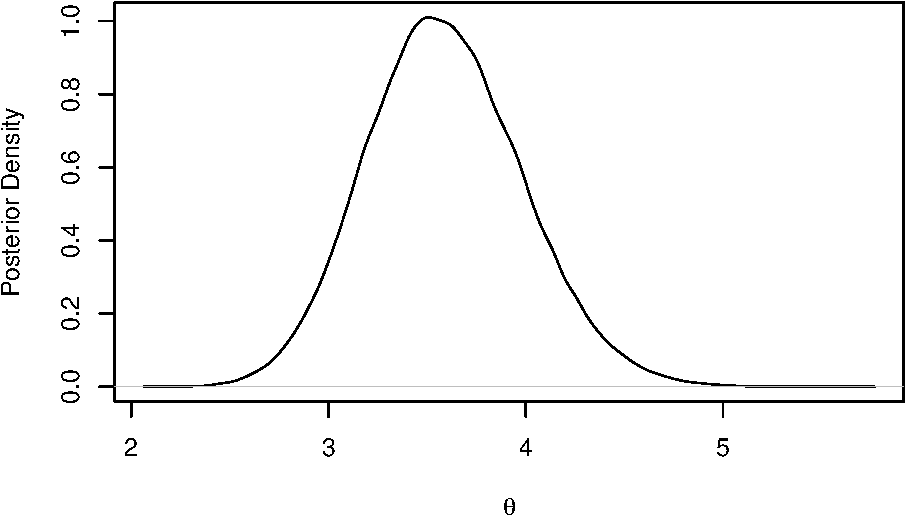
\includegraphics[width=0.75\linewidth]{finalexam_files/figure-latex/ex1-post-density-theta-1} 

}

\caption{The posterior density of the model parameter $\theta$.}\label{fig:ex1-post-density-theta}
\end{figure}

\newpage

\section{Exercise 2}\label{exercise-2}

The data set \texttt{problem2.txt} contains measurements on the annual maximum daily precipitation (mm per 24 hours, from 9:00 AM to 9:00 AM the next day) recorded
at Reykjavík over the years 1926 to 2022. Reykjavík is located in the southwest part of Iceland (64°07.648' N, 21°54.166' W).

\begin{enumerate}[label = (\alph*)]
  \item Assume the data follow a normal distribution, that is
  $$
    Y_i \sim \mathcal N(\mu, \sigma^2), \quad i = 1, \ldots, n,
  $$
  where $\mu \in \mathbb R$, $\sigma^2 > 0$. Assign the following prior densities of $\mu$ and $\sigma^2$,
  $$
    \mu \sim \mathcal N(0, 100^2), \quad \sigma^2 \sim \mathrm{InvGamma}(0.1, 0.1).
  $$
  Sample from the posterior density of $(\mu, \sigma^2)$ by using a Gibbs sampler. Present the formulas for the Gibbs sampler.
  Write code for a Gibbs sampler that samples from the posterior density of $(\mu, \sigma^2)$ (do not use \textsf{JAGS} or other modeling
  libraries). Provide posterior summary for $\mu$ and $\sigma^2$, that is, present the posterior mean, the posterior standard deviation and
  the 95\% equal-tailed posterior interval (based on 4 chains, each of length 13000 with 3000 for burn-in).
  
  \item Plot the theoretical cumulative density function (c.d.f.) of the normal distribution using the posterior means of $\mu$ and $\sigma^2$.
  Plot the empirical cumulative density of the data on the same graph. Does the proposed normal model capture the shape of the empirical cumulative
  density?
  
  \item Draw the trace plots for $\mu$, and $\sigma^2$, using the \texttt{plot} command in \texttt{rjags}. Do these plots indicate that the chains of the two parameters
  are mixing well?
  
  \item Use the \texttt{autocorr.plot} command in \texttt{rjags} to plot the autocorrelation function of each of the sampled parameters. Is the autocorrelation strong or
  weak? Do the autocorrelation functions indicate that  the chains of the parameters will converge quickly or slowly?
  
  \item Compute the following diagnostic statistics: the lag 1 autocorrelation, the effective sample size, and the Gelman-Rubin statistic for each of the
  two parameters. Interpret these diagnostic statistics.
  
  \item Assume here that the data follow a lognormal distribution. This is equivalent to assuming that $U_i = \log(Y_i)$ follows a normal distribution, that is
  $$
    U_i \sim \mathrm{Normal}(\eta, \kappa^2), \quad i = 1, \ldots, n,
  $$
  where $\eta \in \mathbb R$, $\kappa^2 > 0$. Assign the following prior densities to $\eta$ and $\kappa^2$,
  $$
    \eta \sim \mathrm{Normal}(0, 100^2), \quad \kappa^2 \sim \mathrm{InvGamma}(0.1, 0.1).
  $$
  Sample from the posterior density of $(\eta, \kappa^2)$ by using a Gibbs sampler (same formulas as in (a) but a different response variable). Provide posterior
  summary for $\eta$ and $\kappa^2$, that is, present their posterior means, the posterior standard deviations and their equal-tailed posterior intervals (based
  on 4 chains, each of length 13000 with 3000 for burn-in).
  
  \item Plot the theoretical cumulative density function (c.d.f.) of the normal distribution using the posterior means of $\eta$ and $\kappa^2$. Plot the empirical cumulative
  density of the log-transformed data on the same graph. Does the proposed normal model capture the shape of the empirical cumulative density of the log-transformed data?
  
  \item Based on the plots in (b) and (g), which of the two models appears to be better suited for the annual maximum daily precipitation data?

\end{enumerate}

\newpage

\section{Solution}\label{solution-1}

\subsection{Part (a)}\label{part-a-1}

Derivations from the course book show that given the model

\[
  Y_i \sim \mathcal N(\mu, \sigma^2), \quad \mu \sim \mathcal N(\gamma, \tau^2) \quad \text{and} \quad \sigma^2 \sim \mathrm{InvGamma}(\alpha, \beta)
\]
it can be shown that

\begin{align*}
  &\mu | \sigma^2, \mathbf Y \sim \mathcal N\left(\frac{\sum_{i = 1}^n Y_i/\sigma^2 + \gamma/\tau^2}{n/\sigma^2 + 1/\tau^2}, \frac{1}{n/\sigma^2 + 1/\tau^2}\right), \\
  &\sigma^2 | \mu, \mathbf Y \sim \mathrm{InvGamma}\left(n/2 + \alpha, \sum_{i = 1}^n (Y_i - \mu)^2/ 2 + \beta\right).
\end{align*}

Thus, in our case where \(\gamma = 0\), \(\tau^2 = 100^2\), \(\alpha = \beta = 0.1\), the full conditionals for model parameters \(\mu\) and \(\sigma^2\) are given by

\begin{align*}
  &\mu | \sigma^2, \mathbf Y \sim \mathcal N\left(\frac{\sum_{i = 1}^n Y_i / \sigma^2}{n/\sigma^2 + 1/100^2}, \frac{1}{n/\sigma^2 + 1/100^2}\right) \\
  &\sigma^2 | \mu, \mathbf Y \sim \mathrm{InvGamma}\left(n/2 + 0.01, \sum_{i = 1}^n (Y_i - \mu)^2/2 + 0.01\right)
\end{align*}

We now have the formulae needed to set up a Gibbs sampler to summarise the posterior. All that is left is to implement the algorithm in code.

\begin{Shaded}
\begin{Highlighting}[]
\CommentTok{\# set seed for reproducibility}
\FunctionTok{set.seed}\NormalTok{(}\DecValTok{42}\NormalTok{)}

\NormalTok{data2 }\OtherTok{\textless{}{-}} \FunctionTok{read.table}\NormalTok{(}\StringTok{"data/problem2.txt"}\NormalTok{, }\AttributeTok{header=}\NormalTok{T)}
\NormalTok{Y     }\OtherTok{\textless{}{-}}\NormalTok{ data2[,}\DecValTok{2}\NormalTok{] }
\NormalTok{year  }\OtherTok{\textless{}{-}}\NormalTok{ data2[,}\DecValTok{1}\NormalTok{]}

\NormalTok{n }\OtherTok{\textless{}{-}} \FunctionTok{length}\NormalTok{(Y)}

\CommentTok{\# no. samples + burn{-}in}
\NormalTok{burn }\OtherTok{\textless{}{-}} \DecValTok{3000}
\NormalTok{S    }\OtherTok{\textless{}{-}} \FloatTok{1e+4} \SpecialCharTok{+}\NormalTok{ burn}

\NormalTok{compute\_chain }\OtherTok{\textless{}{-}} \ControlFlowTok{function}\NormalTok{() \{}
  
  \CommentTok{\# Create data frame for model params}
\NormalTok{  theta     }\OtherTok{\textless{}{-}} \FunctionTok{matrix}\NormalTok{(}\ConstantTok{NA}\NormalTok{, }\AttributeTok{nrow =}\NormalTok{ S, }\AttributeTok{ncol =} \DecValTok{2}\NormalTok{)}
\NormalTok{  theta[}\DecValTok{1}\NormalTok{,] }\OtherTok{\textless{}{-}} \FunctionTok{c}\NormalTok{(}\FunctionTok{mean}\NormalTok{(Y), }\FunctionTok{var}\NormalTok{(Y))}
  
  \FunctionTok{colnames}\NormalTok{(theta) }\OtherTok{\textless{}{-}} \FunctionTok{c}\NormalTok{(}\StringTok{"mu"}\NormalTok{, }\StringTok{"sigma2"}\NormalTok{)}
  
  \CommentTok{\# Gibbs sampling}
  \ControlFlowTok{for}\NormalTok{ (s }\ControlFlowTok{in} \DecValTok{2}\SpecialCharTok{:}\NormalTok{S) \{}
\NormalTok{    sigma2 }\OtherTok{\textless{}{-}}\NormalTok{ theta[s }\SpecialCharTok{{-}} \DecValTok{1}\NormalTok{, }\StringTok{"sigma2"}\NormalTok{]}
    
\NormalTok{    N }\OtherTok{\textless{}{-}} \FunctionTok{sum}\NormalTok{(Y) }\SpecialCharTok{/}\NormalTok{ sigma2}
\NormalTok{    D }\OtherTok{\textless{}{-}}\NormalTok{ n}\SpecialCharTok{/}\NormalTok{sigma2 }\SpecialCharTok{+} \DecValTok{1}\SpecialCharTok{/}\DecValTok{100}\SpecialCharTok{\^{}}\DecValTok{2}
\NormalTok{    mu  }\OtherTok{\textless{}{-}} \FunctionTok{rnorm}\NormalTok{(}\DecValTok{1}\NormalTok{, }\AttributeTok{mean =}\NormalTok{ N}\SpecialCharTok{/}\NormalTok{D, }\FunctionTok{sqrt}\NormalTok{(D))}

\NormalTok{    A }\OtherTok{\textless{}{-}}\NormalTok{ n}\SpecialCharTok{/}\DecValTok{2} \SpecialCharTok{+} \FloatTok{0.01}
\NormalTok{    B }\OtherTok{\textless{}{-}} \FunctionTok{sum}\NormalTok{((Y }\SpecialCharTok{{-}}\NormalTok{ mu)}\SpecialCharTok{\^{}}\DecValTok{2}\NormalTok{)}\SpecialCharTok{/}\DecValTok{2} \SpecialCharTok{+} \FloatTok{0.01}
\NormalTok{    sig2 }\OtherTok{\textless{}{-}} \FunctionTok{rinvgamma}\NormalTok{(}\DecValTok{1}\NormalTok{, A, B)}
    
\NormalTok{    theta[s,] }\OtherTok{\textless{}{-}} \FunctionTok{c}\NormalTok{(mu, sig2)}
\NormalTok{  \}}
  \FunctionTok{return}\NormalTok{(theta[(burn }\SpecialCharTok{+} \DecValTok{1}\NormalTok{)}\SpecialCharTok{:}\NormalTok{S,])}
\NormalTok{\}}
\end{Highlighting}
\end{Shaded}

Using the \texttt{compute\_chain} function defined above, we can create four chains, convert them into \texttt{mcmc} objects from \texttt{rjags},
and combine them into a \texttt{mcmc.list} which can be summarised using functions from \texttt{rjags}.

\begin{Shaded}
\begin{Highlighting}[]
\NormalTok{chains }\OtherTok{\textless{}{-}} \FunctionTok{lapply}\NormalTok{(}\DecValTok{1}\SpecialCharTok{:}\DecValTok{4}\NormalTok{, }\ControlFlowTok{function}\NormalTok{(i) }\FunctionTok{mcmc}\NormalTok{(}\FunctionTok{compute\_chain}\NormalTok{()))}
\NormalTok{chains\_jags }\OtherTok{\textless{}{-}} \FunctionTok{mcmc.list}\NormalTok{(chains)}
\NormalTok{sum\_jags }\OtherTok{\textless{}{-}} \FunctionTok{summary}\NormalTok{(chains\_jags)}

\NormalTok{sum\_jags}
\end{Highlighting}
\end{Shaded}

\begin{verbatim}
## 
## Iterations = 1:10000
## Thinning interval = 1 
## Number of chains = 4 
## Sample size per chain = 10000 
## 
## 1. Empirical mean and standard deviation for each variable,
##    plus standard error of the mean:
## 
##         Mean     SD Naive SE Time-series SE
## mu     31.29  1.136  0.00568       0.005591
## sigma2 78.13 11.670  0.05835       0.057471
## 
## 2. Quantiles for each variable:
## 
##         2.5%   25%   50%   75%  97.5%
## mu     29.07 30.53 31.29 32.06  33.54
## sigma2 58.61 69.81 77.02 85.19 104.00
\end{verbatim}

From the summary output above one sees that the posterior mean for \(\mu\) is 30.64, with posterior standard deviation \(0.8256\) and 95\% credible set \([29.02, 32.28]\). The full summary of the model parameters are shown below in Table 2.

\begin{table}[H]
  \centering
  \begin{tabular}{clll}
    \toprule
          & Mean & Standard deviation & 95\% credible set \\
    \midrule
    $\mu$      & 31.2923739 &  1.1359336 & $[29.0727376, 33.543175]$ \\
    $\sigma^2$ & 78.1299623 &  11.6695249 & $[58.6128057, 104.0041172]$ \\
    \bottomrule
  \end{tabular}
  \label{ex2-sum-stats}
  \caption{Summary statistics for parameters $\mu$ and $\sigma^2$ in the model.}
\end{table}

\newpage

\subsection{Part (b)}\label{part-b-1}

Figure \ref{fig:ex2-ecdf-vs-theory} shows a comparisonal plot of the empirical cumulative density function of the precipitation data compared with the theoretical c.d.f. which was constructed using the posterior mean estimates of model parameters \(\mu\) and \(\sigma^2\). Judging from the graph, it seems like the normal model is able to capture patterns in the data with considerable accuracy.

\begin{figure}

{\centering 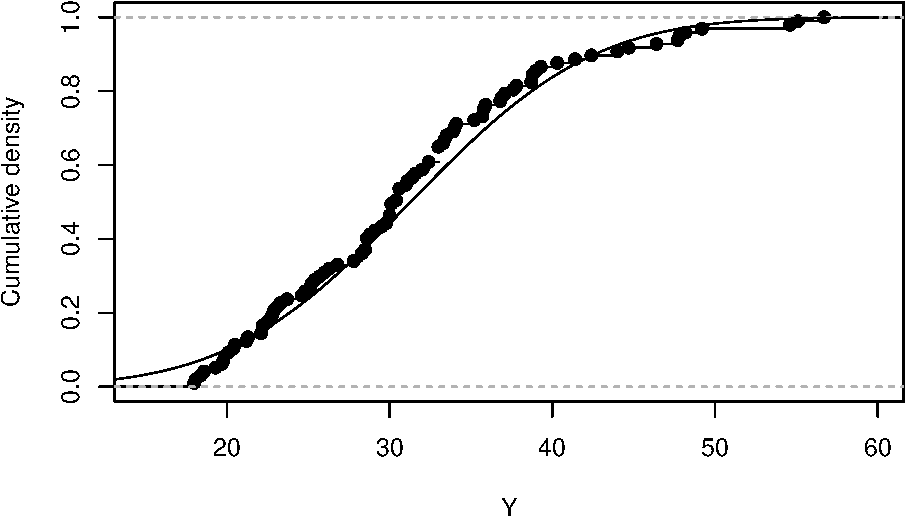
\includegraphics[width=0.75\linewidth]{finalexam_files/figure-latex/ex2-ecdf-vs-theory-1} 

}

\caption{Empirical and theoretical cumulative density functions.}\label{fig:ex2-ecdf-vs-theory}
\end{figure}

\subsection{Part (c)}\label{part-c-1}

Trace and density plots of model parameters \(\mu\) and \(\sigma^2\) are shown in Figure \ref{fig:ex2-trace-plots}. Linear structure in the trace plots is indicative of the fact that the parameter estimates converge to a probabilistic centre (some prefer to describe the
structure as caterpillar or barcode-like). Thus the parameters seems to be mixing well.

\begin{figure}

{\centering 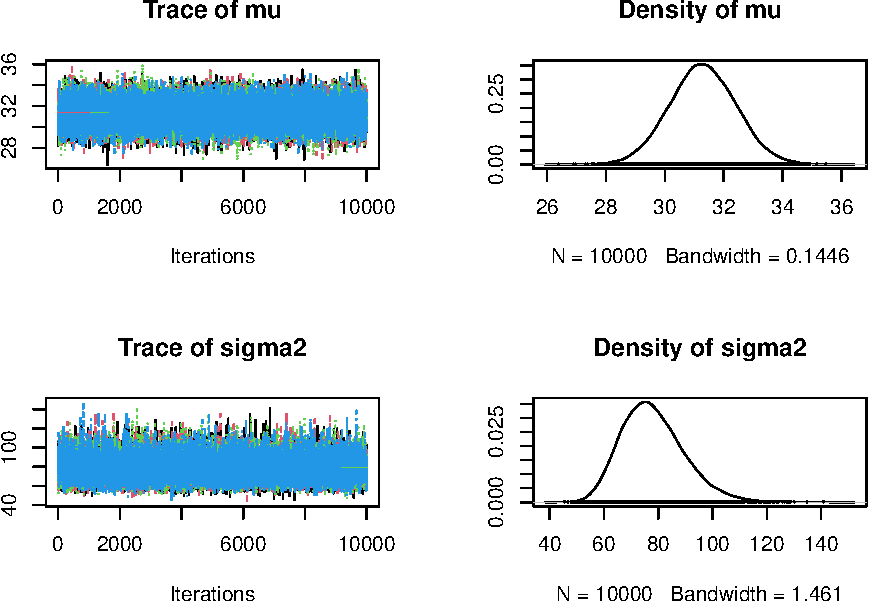
\includegraphics[width=0.7\linewidth]{finalexam_files/figure-latex/ex2-trace-plots-1} 

}

\caption{Trace plots of model parameters $\mu$ and $\sigma^2$ in the normal model.}\label{fig:ex2-trace-plots}
\end{figure}
\newpage

\subsection{Part (d)}\label{part-d}

Figure \ref{fig:ex2-autocorr-plots} shows autocorrelation plots for each of the chains generated in part (a).
The first line of the plots shows the autocorrelation plots for the first chain, and so forth. The graphs show very little
correlation besides at lag \(\ell = 0\) which is obviously to be expected. This implies a rapid rate of convergence, since for
lag \(\ell > 0\) it seems that the dependence or correlation between samples is very little at best, indicating that the samples
being drawn from the posterior almost instantly become independent. One could raise point out that this autocorrelation analysis
was performed on burned-in samples and investigating the raw samples would be more appropriate, but they yield the exact same
results since we picked good initial values.

\begin{center}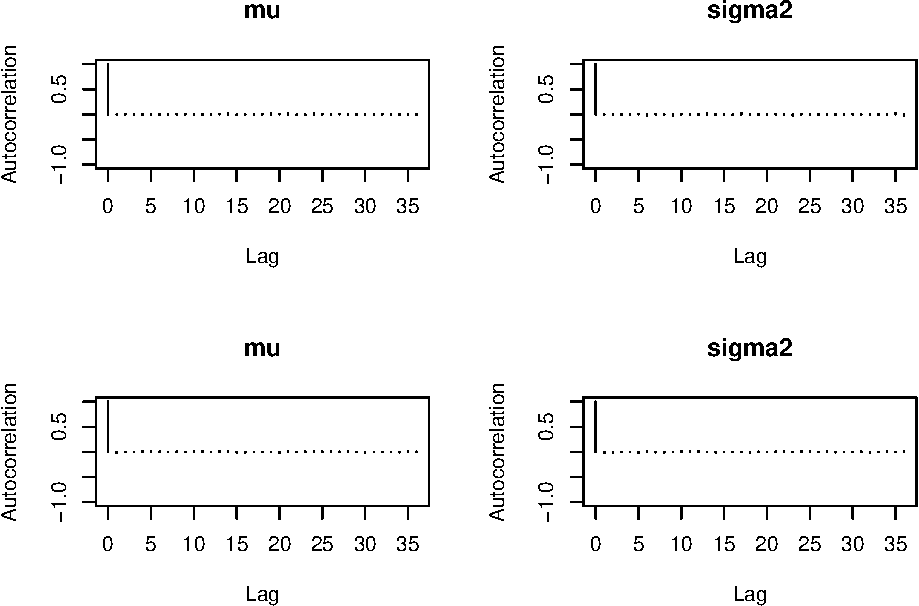
\includegraphics[width=0.75\linewidth]{finalexam_files/figure-latex/unnamed-chunk-6-1} \end{center}

\begin{figure}

{\centering 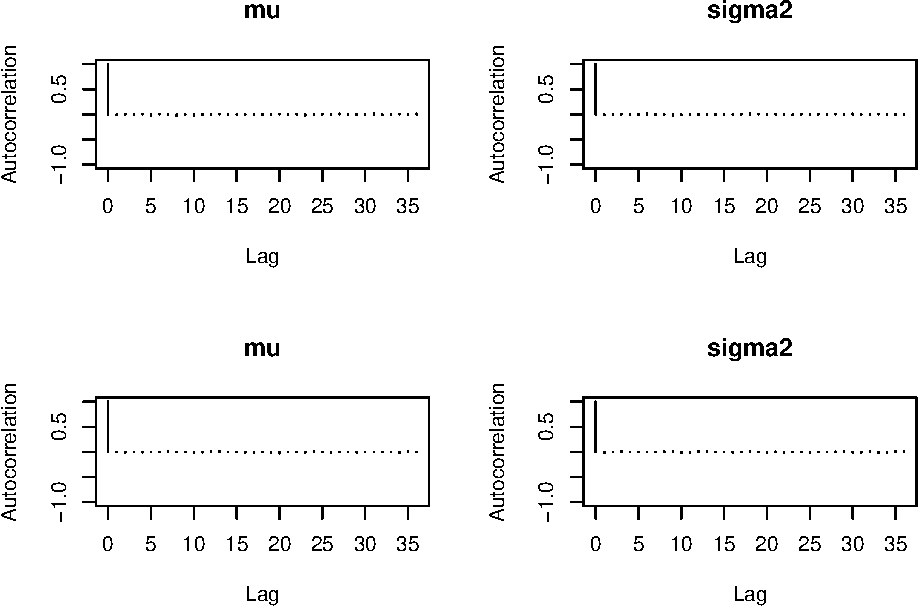
\includegraphics[width=0.75\linewidth]{finalexam_files/figure-latex/ex2-autocorr-plots-1} 

}

\caption{Autocorrelation plots for the chains generated in part (a).}\label{fig:ex2-autocorr-plots}
\end{figure}

\newpage

\subsection{Part (e)}\label{part-e}

Start with the autocorrelation with \(\ell = 1\):

\begin{Shaded}
\begin{Highlighting}[]
\FunctionTok{autocorr.diag}\NormalTok{(chains\_jags, }\AttributeTok{lag =} \DecValTok{1}\NormalTok{)}
\end{Highlighting}
\end{Shaded}

\begin{verbatim}
##                 mu      sigma2
## Lag 1 -0.007896202 -0.01662788
\end{verbatim}

There is very little correlation between samples for both \(\mu\) and \(\sigma^2\), virtually none. This indicates that for a given sample, its predecessor has gives no bearing on how its successor evolves,
which implies that the assumption of independent sampling holds. Let us next look at the effective sample size diagnostic:

\begin{Shaded}
\begin{Highlighting}[]
\FunctionTok{effectiveSize}\NormalTok{(chains\_jags)}
\end{Highlighting}
\end{Shaded}

\begin{verbatim}
##       mu   sigma2 
## 41304.98 41245.44
\end{verbatim}

In both cases it is very high, exceeding the ``couple thousand'' rule-of-thumb threshold for all parameters. In fact, it is centred around the Monte Carlo sample size \(S\) which
was used in the code for the Gibbs sampler, which implies that the information per sample contained in the samples in the four chains is one-to-one. Thus there is no redundancy
in the samples which is equivalent to the samples being uncorrelated (this also follows from the definition of the \(ESS\) diagnostic). Finish with the Gelman-Rubin diagnostic:

\begin{Shaded}
\begin{Highlighting}[]
\FunctionTok{gelman.diag}\NormalTok{(chains\_jags)}
\end{Highlighting}
\end{Shaded}

\begin{verbatim}
## Potential scale reduction factors:
## 
##        Point est. Upper C.I.
## mu              1          1
## sigma2          1          1
## 
## Multivariate psrf
## 
## 1
\end{verbatim}

In similar fashion, Gelman-Rubin diagnostic indicates excellent convergence. The Gelman-Rubin diagnostic is essentially the scaled result of an ANOVA test which compares the
means between chains, or in other words whether they agree. In this case it is evident.

\subsection{Part (f)}\label{part-f}

The Gibbs sampler is set up below, this time using \textsf{JAGS} for convenience:

\begin{Shaded}
\begin{Highlighting}[]
\NormalTok{init\_log }\OtherTok{\textless{}{-}} \FunctionTok{textConnection}\NormalTok{(}\StringTok{"model\{}
\StringTok{  for (i in 1:n) \{}
\StringTok{    Y[i] \textasciitilde{} dlnorm(eta, tau)}
\StringTok{  \}}
\StringTok{  }
\StringTok{  eta \textasciitilde{} dnorm(0, 0.0001)}
\StringTok{  tau \textasciitilde{} dgamma(0.1, 0.1)}
\StringTok{  kappa \textless{}{-} 1/tau}
\StringTok{\}"}\NormalTok{)}

\NormalTok{model\_log }\OtherTok{\textless{}{-}} \FunctionTok{jags.model}\NormalTok{(init\_log, }\AttributeTok{data =} \FunctionTok{list}\NormalTok{(}\AttributeTok{Y =}\NormalTok{ Y, }\AttributeTok{n =}\NormalTok{ n), }\AttributeTok{n.chains =} \DecValTok{4}\NormalTok{, }\AttributeTok{quiet =} \ConstantTok{TRUE}\NormalTok{)}
\FunctionTok{update}\NormalTok{(model\_log, }\AttributeTok{n.iter =} \DecValTok{3000}\NormalTok{, }\AttributeTok{progress.bar =} \StringTok{"none"}\NormalTok{)}
\NormalTok{samples\_log }\OtherTok{\textless{}{-}} \FunctionTok{coda.samples}\NormalTok{(model\_log, }\AttributeTok{variable.names =} \FunctionTok{c}\NormalTok{(}\StringTok{"eta"}\NormalTok{, }\StringTok{"kappa"}\NormalTok{), }\AttributeTok{n.iter =} \DecValTok{10000}\NormalTok{, }
                            \AttributeTok{progress.bar =} \StringTok{"none"}\NormalTok{)}
\end{Highlighting}
\end{Shaded}

\begin{figure}

{\centering 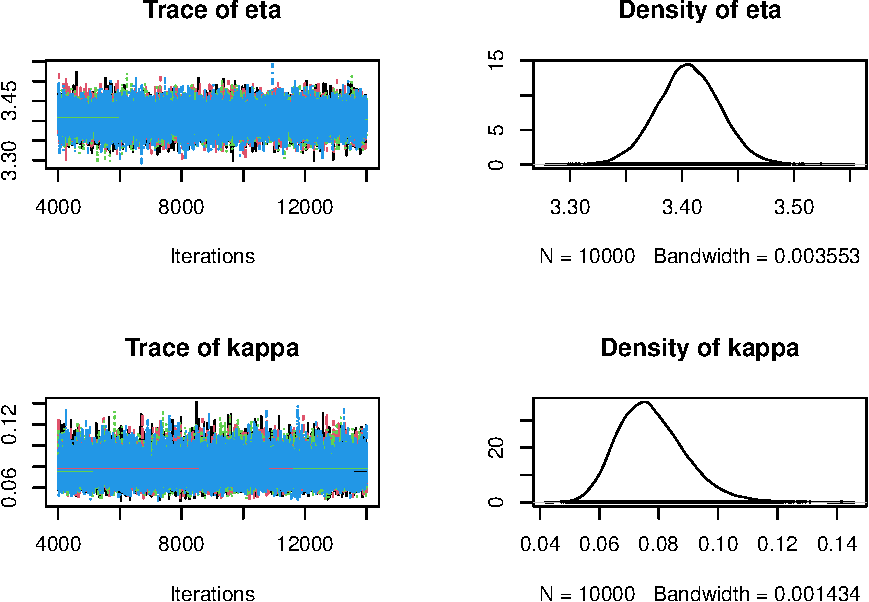
\includegraphics[width=0.75\linewidth]{finalexam_files/figure-latex/ex2-log-trace-1} 

}

\caption{Trace and density plots of model parameters $\eta$ and $\kappa^2$ in the log-normal model.}\label{fig:ex2-log-trace}
\end{figure}

Figure \ref{fig:ex2-log-trace} shows trace and density plots of model parameters \(\eta\) and \(\kappa^2\). The chains are obviously convergent.
Let us look at some summary statistics for the log-normal model, also shown in Table 3.

\begin{Shaded}
\begin{Highlighting}[]
\NormalTok{sum\_precip }\OtherTok{\textless{}{-}} \FunctionTok{summary}\NormalTok{(samples\_log)}
\NormalTok{sum\_precip}
\end{Highlighting}
\end{Shaded}

\begin{verbatim}
## 
## Iterations = 4001:14000
## Thinning interval = 1 
## Number of chains = 4 
## Sample size per chain = 10000 
## 
## 1. Empirical mean and standard deviation for each variable,
##    plus standard error of the mean:
## 
##          Mean      SD  Naive SE Time-series SE
## eta   3.40598 0.02835 0.0001417      0.0001838
## kappa 0.07774 0.01146 0.0000573      0.0000572
## 
## 2. Quantiles for each variable:
## 
##          2.5%     25%     50%     75%  97.5%
## eta   3.34963 3.38738 3.40584 3.42478 3.4621
## kappa 0.05852 0.06957 0.07657 0.08466 0.1034
\end{verbatim}

\begin{table}[H]
  \centering
  \begin{tabular}{clll}
    \toprule
          & Mean & Standard deviation & 95\% credible set \\
    \midrule
    $\eta$      & 3.4059848 & 0.0283456 & $[3.3496337, 3.4621452]$ \\
    $\kappa^2$  & 0.0777426 & 0.0114592 & $[0.0585218, 0.103382]$ \\
    \bottomrule
  \end{tabular}
  \label{tab:ex2-sum-stats-log}
  \caption{Summary statistics for parameters $\eta$ and $\kappa^2$ in the log-normal model, rounded to two decimals.}
\end{table}

\subsection{Part (g)}\label{part-g}

Figure \ref{fig:ex2-log-ecdf} shows the empirical and theoretical cumulative density functions.

\begin{figure}

{\centering 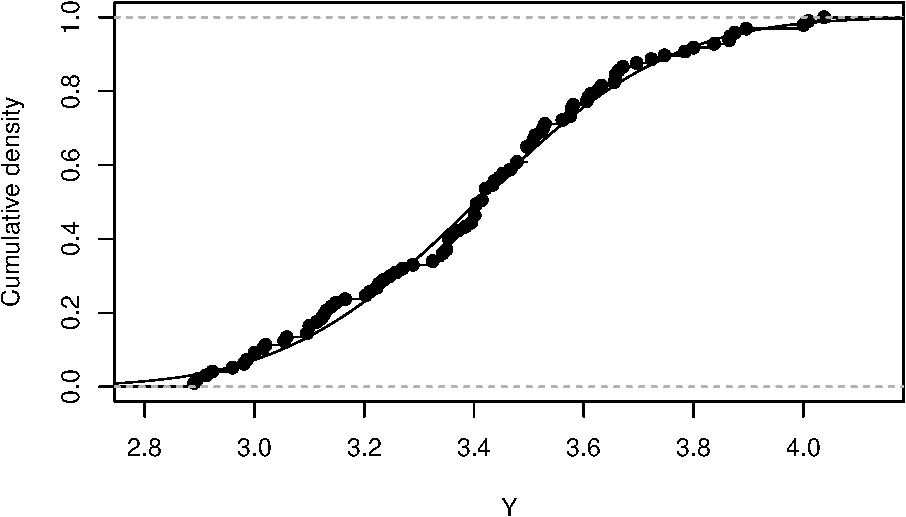
\includegraphics[width=0.75\linewidth]{finalexam_files/figure-latex/ex2-log-ecdf-1} 

}

\caption{Empirical and theoretical cumulative density functions in the log-normal model.}\label{fig:ex2-log-ecdf}
\end{figure}

\subsection{Part (h)}\label{part-h}

A comparison of Figures \ref{fig:ex2-ecdf-vs-theory} and \ref{fig:ex2-log-ecdf} shows that the discrepancy is lessened when working with the log-transformed data,
i.e.~the difference between the empirical cumulative density and the theoretical one is more similar in the log-normal model. Therefore, this model is preferrable to
the one using the untransformed data.

\begin{figure}

{\centering 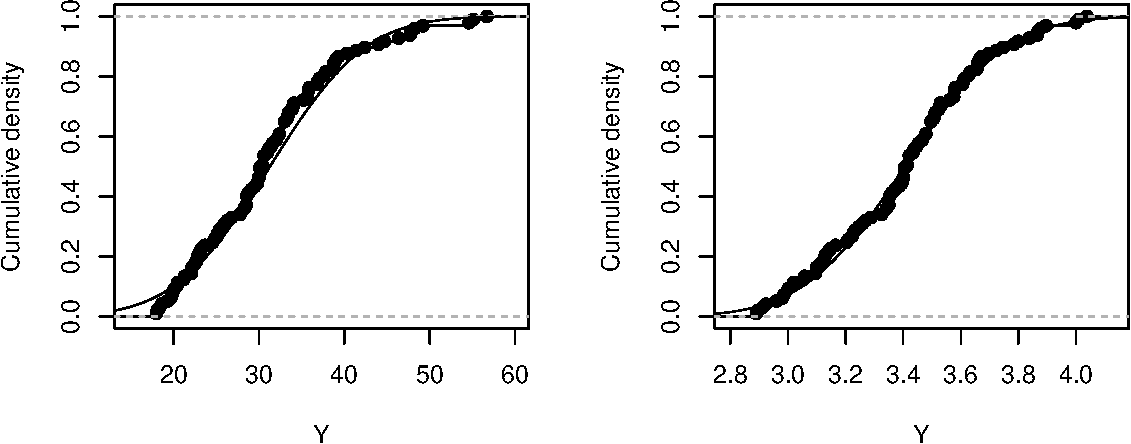
\includegraphics[width=1\linewidth]{finalexam_files/figure-latex/ex2-cmp-normal-models-1} 

}

\caption{Visual comparison of the untransformed and log-normal models.}\label{fig:ex2-cmp-normal-models}
\end{figure}

\newpage

\section{Exercise 3}\label{exercise-3}

Here we explore two methods to compare proportions of individuals with a particular trait in two populations, namely DIC and Bayes factor. Assume that we have
independent samples from each of the populations, and the sample sizes are \(n_1 = 1053\) and \(n_2 = 976\), respectively. Let \(Y_j\) denote the number of individuals
with the trait in the sample from population \(j \in \{1, 2\}\). Assume that the samples are such that \(Y_1 = 26\) and \(Y_2 = 45\).

To compare the two proportions, we compare two models. Model 1, \(\mathcal M_1\), is such that
\[
  Y_1 \sim \mathrm{Bin}(n_1, \theta), \quad Y_2 \sim \mathrm{Bin}(n_2, \theta), \quad \theta \sim \mathrm{Beta}(1, 1).
\]
Model 2, \(\mathcal M_2\), is such that
\[
  Y_1 \sim \mathrm{Bin}(n_1, \theta_1), \quad Y_2 \sim \mathrm{Bin}(n_2, \theta_2), \quad \theta_1 \sim \mathrm{Beta}(1, 1), \quad \theta_2 \sim \mathrm{Beta}(1, 1).
\]

\begin{enumerate}[label = (\alph*)]
  \item Use DIC to compare the two models. Use simulation to estimate DIC for each of the two models.
  In the case of the above data, does the difference in DIC indicate that Model 2 is a more suitable model?
  
  \item Use Bayes factor to compare the models. Assume \emph{a priori} that the two models are equally likely.
  Here we use the result for Bayes factor directly. The Bayes factor of Model 2 relative to Model 1 is given by
  $$
    \mathrm{BF} = \frac{Y_1!(n_1 - Y_1)! Y_2!(n_2 - Y_2)! (n_1 + n_2 + 1)!}{(n_1 + 1)! (n_2 + 1)! (Y_1 + Y_2)! (n_1 + n_2 - Y_1 - Y_2)!}.
  $$
  In the case of the above data, does the value of BF indicate that Model 2 is a more suitable model?
  
  \item Derive the formula for the Bayes factor given in (b).
\end{enumerate}

\section{Solution}\label{solution-2}

\subsection{Part (a)}\label{part-a-2}

The code for comparing the models via DIC is shown below.

\begin{Shaded}
\begin{Highlighting}[]
\NormalTok{n }\OtherTok{\textless{}{-}} \FunctionTok{c}\NormalTok{(}\DecValTok{1053}\NormalTok{, }\DecValTok{976}\NormalTok{)}
\NormalTok{Y }\OtherTok{\textless{}{-}} \FunctionTok{c}\NormalTok{(}\DecValTok{26}\NormalTok{, }\DecValTok{45}\NormalTok{)}

\NormalTok{init\_M1 }\OtherTok{\textless{}{-}} \FunctionTok{textConnection}\NormalTok{(}\StringTok{"model\{}
\StringTok{  for (i in 1:2) \{ }
\StringTok{    Y[i] \textasciitilde{} dbin(theta, n[i]) }
\StringTok{  \}}
\StringTok{  theta \textasciitilde{} dbeta(1, 1)}
\StringTok{\}"}\NormalTok{)}

\NormalTok{init\_M2 }\OtherTok{\textless{}{-}} \FunctionTok{textConnection}\NormalTok{(}\StringTok{"model\{}
\StringTok{  for (i in 1:2) \{ }
\StringTok{    Y[i] \textasciitilde{} dbin(theta[i], n[i]) }
\StringTok{    theta[i] \textasciitilde{} dbeta(1, 1)}
\StringTok{  \}}
\StringTok{\}"}\NormalTok{)}

\NormalTok{data }\OtherTok{\textless{}{-}} \FunctionTok{list}\NormalTok{(}\AttributeTok{n =}\NormalTok{ n, }\AttributeTok{Y =}\NormalTok{ Y)}

\NormalTok{model\_M1 }\OtherTok{\textless{}{-}} \FunctionTok{jags.model}\NormalTok{(init\_M1, }\AttributeTok{data =}\NormalTok{ data, }\AttributeTok{n.chains =} \DecValTok{2}\NormalTok{, }\AttributeTok{quiet =} \ConstantTok{TRUE}\NormalTok{)}
\NormalTok{model\_M2 }\OtherTok{\textless{}{-}} \FunctionTok{jags.model}\NormalTok{(init\_M2, }\AttributeTok{data =}\NormalTok{ data, }\AttributeTok{n.chains =} \DecValTok{2}\NormalTok{, }\AttributeTok{quiet =} \ConstantTok{TRUE}\NormalTok{)}

\FunctionTok{update}\NormalTok{(model\_M1, }\AttributeTok{n.iter =} \DecValTok{3000}\NormalTok{, }\AttributeTok{progress.bar =} \StringTok{"none"}\NormalTok{)}
\FunctionTok{update}\NormalTok{(model\_M2, }\AttributeTok{n.iter =} \DecValTok{3000}\NormalTok{, }\AttributeTok{progress.bar =} \StringTok{"none"}\NormalTok{)}

\NormalTok{DIC\_M1 }\OtherTok{\textless{}{-}} \FunctionTok{dic.samples}\NormalTok{(model\_M1, }\AttributeTok{n.iter =} \DecValTok{10000}\NormalTok{, }\AttributeTok{progress.bar =} \StringTok{"none"}\NormalTok{)}
\NormalTok{DIC\_M2 }\OtherTok{\textless{}{-}} \FunctionTok{dic.samples}\NormalTok{(model\_M2, }\AttributeTok{n.iter =} \DecValTok{10000}\NormalTok{, }\AttributeTok{progress.bar =} \StringTok{"none"}\NormalTok{)}

\NormalTok{DIC\_M1; DIC\_M2}
\end{Highlighting}
\end{Shaded}

\begin{verbatim}
## Mean deviance:  18.6 
## penalty 0.975 
## Penalized deviance: 19.58
\end{verbatim}

\begin{verbatim}
## Mean deviance:  12.67 
## penalty 1.984 
## Penalized deviance: 14.66
\end{verbatim}

From the output we see that \(\mathrm{DIC}_{\mathcal M_1} = 19.58\) and \(\mathrm{DIC}_{\mathcal M_2} = 14.66\). This indicates that model \(\mathcal M_2\) is favoured.
We can verify this by comparing the result rendered by frequentist proportion test:

\begin{Shaded}
\begin{Highlighting}[]
\FunctionTok{prop.test}\NormalTok{(Y, n)}
\end{Highlighting}
\end{Shaded}

\begin{verbatim}
## 
##  2-sample test for equality of proportions with continuity correction
## 
## data:  Y out of n
## X-squared = 6.2596, df = 1, p-value = 0.01235
## alternative hypothesis: two.sided
## 95 percent confidence interval:
##  -0.038556503 -0.004273895
## sample estimates:
##     prop 1     prop 2 
## 0.02469136 0.04610656
\end{verbatim}

Again the test concludes that \(\mathcal M_2\) is favourable (or from a frequentist perspective, that the proportions are inequal between groups), but the result is not decisive as
can be seen from the \(p\)-value of the test.

\subsection{Part (b)}\label{part-b-2}

The Bayes factor for comparing the two models is given by
\[
  \mathrm{BF} = \frac{\Pr(\mathcal M_2 | \mathbf Y) / \Pr(\mathcal M_1 | \mathbf Y)}{\Pr(\mathcal M_2) / \Pr(\mathcal M_1)} = \frac{\Pr(\mathcal M_2 | \mathbf Y)}{\Pr(\mathcal M_1 | \mathbf Y)}
\]
where the expression was reduced to the form to the right in light of the fact that \(\Pr(\mathcal M_1) = \Pr(\mathcal M_2)\). Also, it is known to be

\begin{align*}
    \mathrm{BF} &= \frac{Y_1!(n_1 - Y_1)! Y_2!(n_2 - Y_2)! (n_1 + n_2 + 1)!}{(n_1 + 1)! (n_2 + 1)! (Y_1 + Y_2)! (n_1 + n_2 - Y_1 - Y_2)!} \\
                &= \frac{\Gamma(Y_1 + 1) \Gamma(n_1 - Y_1 + 1) \Gamma(Y_2 + 1) \Gamma(n_2 - Y_2 + 1) \Gamma(n_1 + n_2 + 2)}{\Gamma(n_1 + 2) \Gamma(n_2 + 2) \Gamma(Y_1 + Y_2 + 1) \Gamma(n_1 + n_2 - Y_1 - Y_2 + 1)}
\end{align*}

since \(\Gamma(x + 1) = x!\). So computing the Bayes factor for \(\mathcal M_1\) and \(\mathcal M_2\) can be carried out as follows:

\begin{Shaded}
\begin{Highlighting}[]
\NormalTok{numer }\OtherTok{\textless{}{-}} \FunctionTok{lgamma}\NormalTok{(Y[}\DecValTok{1}\NormalTok{] }\SpecialCharTok{+} \DecValTok{1}\NormalTok{) }\SpecialCharTok{+} \FunctionTok{lgamma}\NormalTok{(n[}\DecValTok{1}\NormalTok{] }\SpecialCharTok{{-}}\NormalTok{ Y[}\DecValTok{1}\NormalTok{] }\SpecialCharTok{+} \DecValTok{1}\NormalTok{) }\SpecialCharTok{+} \FunctionTok{lgamma}\NormalTok{(Y[}\DecValTok{2}\NormalTok{] }\SpecialCharTok{+} \DecValTok{1}\NormalTok{) }\SpecialCharTok{+} 
         \FunctionTok{lgamma}\NormalTok{(n[}\DecValTok{2}\NormalTok{] }\SpecialCharTok{{-}}\NormalTok{ Y[}\DecValTok{2}\NormalTok{] }\SpecialCharTok{+} \DecValTok{1}\NormalTok{) }\SpecialCharTok{+} \FunctionTok{lgamma}\NormalTok{(n[}\DecValTok{1}\NormalTok{] }\SpecialCharTok{+}\NormalTok{ n[}\DecValTok{2}\NormalTok{] }\SpecialCharTok{+} \DecValTok{2}\NormalTok{)}
\NormalTok{denom }\OtherTok{\textless{}{-}} \FunctionTok{lgamma}\NormalTok{(n[}\DecValTok{1}\NormalTok{] }\SpecialCharTok{+} \DecValTok{2}\NormalTok{) }\SpecialCharTok{+} \FunctionTok{lgamma}\NormalTok{(n[}\DecValTok{2}\NormalTok{] }\SpecialCharTok{+} \DecValTok{2}\NormalTok{) }\SpecialCharTok{+} \FunctionTok{lgamma}\NormalTok{(Y[}\DecValTok{1}\NormalTok{] }\SpecialCharTok{+}\NormalTok{ Y[}\DecValTok{2}\NormalTok{] }\SpecialCharTok{+} \DecValTok{1}\NormalTok{) }\SpecialCharTok{+} 
         \FunctionTok{lgamma}\NormalTok{(n[}\DecValTok{1}\NormalTok{] }\SpecialCharTok{+}\NormalTok{ n[}\DecValTok{2}\NormalTok{] }\SpecialCharTok{{-}}\NormalTok{ Y[}\DecValTok{1}\NormalTok{] }\SpecialCharTok{{-}}\NormalTok{ Y[}\DecValTok{2}\NormalTok{] }\SpecialCharTok{+} \DecValTok{1}\NormalTok{)}
\NormalTok{res }\OtherTok{\textless{}{-}} \FunctionTok{exp}\NormalTok{(numer }\SpecialCharTok{{-}}\NormalTok{ denom)}
\NormalTok{res}
\end{Highlighting}
\end{Shaded}

\begin{verbatim}
## [1] 0.6331682
\end{verbatim}

Interestingly, the Bayes factor of \(\mathcal M_2\) relative to \(\mathcal M_1\) seems to slightly favour the simpler model, \(\mathcal M_1\).

\subsection{Part (c)}\label{part-c-2}

Start by deriving the quantity in the denominator:
\begin{align*}
  \Pr(\mathcal M_1 | \mathbf Y) 
  &= \int_{\Omega} \Pr(\mathcal M_1, \mathbf Y) \, d\theta \\ 
  &= \int_\Omega \mathcal L(\mathbf Y | \mathcal M_1) \pi(\mathcal M_1) \, d\theta \\
  &= \int_\Omega \mathcal L(Y_1 | \mathcal M_1) \mathcal L(Y_2 | \mathcal M_1) \pi(\mathcal M_1) \, d\theta \\
  &= \int_\Omega \binom{n_1}{Y_1} \theta^{Y_1} (1 - \theta)^{n_1 - Y_1} \binom{n_2}{Y_2} \theta^{Y_2} (1 - \theta)^{n_2 - Y_2} \, d\theta \\
  &= \binom{n_1}{Y_1} \binom{n_2}{Y_2} \int_\Omega \theta^{(Y_1 + Y_2 + 1) - 1} (1 - \theta)^{(n_1 + n_2 - Y_1 - Y_2 + 1) - 1} \, d\theta \\
  &= \binom{n_1}{Y_1} \binom{n_2}{Y_2} \frac{\Gamma(Y_1 + Y_2 + 1) \Gamma(n_1 + n_2 - Y_1 - Y_2 + 1)}{\Gamma(n_1 + n_2 + 2)} \int_\Omega \mathcal L(\vartheta | \alpha, \beta) \, d\vartheta \\
  &= \binom{n_1}{Y_1} \binom{n_2}{Y_2} \frac{\Gamma(Y_1 + Y_2 + 1) \Gamma(n_1 + n_2 - Y_1 - Y_2 + 1)}{\Gamma(n_1 + n_2 + 2)}
\end{align*}

where \(\vartheta \sim \mathrm{Beta}(\alpha, \beta)\) such that \(\alpha = Y_1 + Y_2 + 1\) and \(\beta = n_1 + n_2 - Y_1 - Y_2 + 1\). The constant induced by the prior \(\pi(\mathcal M_i)\) is equal to one since \(\Gamma(a + b) = \Gamma(2) = 1\) and \(\Gamma(a)\Gamma(b) = \Gamma(1)^2 = 1\). Move on to the numerator:
\begin{align*}
  \Pr(\mathcal M_2 | \mathbf Y)
  &= \iint_{\boldsymbol\Omega} \Pr(\mathcal M_2, \mathbf Y) \, d\boldsymbol\theta \\
  &= \iint_{\boldsymbol\Omega} \mathcal L(\mathbf Y | \mathcal M_2) \pi(\mathcal M_2) \, d\boldsymbol\theta \\
  &= \int_{\Omega_1} \mathcal L(Y_1 | \mathcal M_2) \pi(\mathcal M_2) \, d\theta_1 \int_{\Omega_2} \mathcal L(Y_2 | \mathcal M_2) \pi(\mathcal M_2) \, d\theta_2 \\
  &= \int_{\Omega_1} \binom{n_1}{Y_1} \theta_1^{Y_1} (1 - \theta_1)^{n_1 - Y_1} \, d\theta_1 \int_{\Omega_2} \binom{n_2}{Y_2} \theta_2^{Y_2} (1 - \theta_2)^{n_2 - Y_2} \, d\theta_2 \\
  &= \binom{n_1}{Y_1}\binom{n_2}{Y_2} \int_{\Omega_1} \theta_1^{(Y_1 + 1) - 1} (1 - \theta)^{(n_1 - Y_1 + 1) - 1} \, d\theta_1 \int_{\Omega_2} \theta^{(Y_2 + 1) - 1} (1 - \theta)^{(n_2 - Y_2 + 1) - 1} \, d\theta_2 \\
  &= \binom{n_1}{Y_1}\binom{n_2}{Y_2} \frac{\Gamma(Y_1 + 1)\Gamma(n_1 - Y_1 + 1)}{\Gamma(n_1 + 2)} \frac{\Gamma(Y_2 + 1)\Gamma(n_2 - Y_2 + 1)}{\Gamma(n_2 + 2)} \int_{\Omega_1} \mathcal L(\vartheta_1 | \boldsymbol\alpha_1) \, d\vartheta_1 \int_{\Omega_2} \mathcal L(\vartheta_2 | \boldsymbol\alpha_2) \, d\vartheta_2 \\
  &= \binom{n_1}{Y_1} \binom{n_2}{Y_2} \frac{\Gamma(Y_1 + 1)\Gamma(n_1 - Y_1 + 1)\Gamma(Y_2 + 1)\Gamma(n_2 - Y_2 + 1)}{\Gamma(n_1 + 2)\Gamma(n_2 + 2)}
\end{align*}
where \(\vartheta_1\) and \(\vartheta_2\) are Beta-distributed random variables with parameters \(\boldsymbol\alpha_1\) and \(\boldsymbol\alpha_2\), respectively. Now,

\[
\mathrm{BF} = \frac{\Pr(\mathcal M_2 | \mathbf Y)}{\Pr(\mathcal M_1 | \mathbf Y)} = \frac{\Gamma(Y_1 + 1) \Gamma(n_1 - Y_1 + 1) \Gamma(Y_2 + 1) \Gamma(n_2 - Y_2 + 1) \Gamma(n_1 + n_2 + 2)}{\Gamma(n_1 + 2) \Gamma(n_2 + 2) \Gamma(Y_1 + Y_2 + 1) \Gamma(n_1 + n_2 - Y_1 - Y_2 + 1)},
\]

which is what we wanted to show.

\newpage

\section{Exercise 4}\label{exercise-4}

For one year, the consumption of petrol, \(Y\) (in millions of gallons) was measured in 48 states. The variables that may affect the consumption of petrol are; the petrol tax, \(X_2\)
(in cents per gallon); the per capita income, \(X_3\) (in 1000 dollars per month); the number of miles of paved highway, \(X_4\) (in 1000 miles); and the percentage of the population with
driver's licenses, \(X_5\). The file \texttt{problem4.txt} contains data of these variables. The columns contain \(X_2\), \(X_3\), \(X_4\), \(X_5\) and \(Y\), respectively.

The following linear model is proposed

\[
  Y_i = \sum_{j = 1}^5 X_{ij} \beta_j + \varepsilon_i, \quad i = 1, \ldots, 48
\]

with \(X_{i1} = 1\) for all \(i\). Assume that the \(Y\)s are independent, normally distributed and have equal variance, that is

\[
  Y_i | \beta_1, \ldots, \beta_5, \sigma^2 \sim \mathcal{N}\left(\sum_{j = 1}^5 X_{ij} \beta_j, \sigma^2\right), \quad i = 1, \ldots, 48
\]

\emph{A priori}, the \(\beta_j\)s are independent of each other, and the prior distribution for each \(\beta_j\) is such that \(\beta_j \sim \mathcal N(0, 100^2)\).
The prior distribution of \(\sigma^2\) is such that \(\sigma^2 \sim \mathrm{InvGamma}(0.1, 0.1)\).

\begin{enumerate}[label = (\alph*)]
  \item Plot $Y$ versus $X_2, X_3, \ldots, X_5$, a total of 4 figures. Which explanatory variables show a clear relationship with $Y$, and which do not?
  
  \item The per capita income, $X_3$, and the percentage of the population with driver's licenses, $X_5$, are known to have an effect on the consumption of
  petrol, $Y$. The effect of the petrol tax, $X_2$, and the number of miles of paved highway, $X_4$, is not as clear. Therefore we test 4 models for the
  mean, namely
  \begin{alignat*}{2}
    &\mathcal M_1: \mu_i = \beta_1 + X_{i3}\beta_3 + X_{i5}\beta_5, \quad &&\mathcal M_2: \mu_i = \beta_1 + X_{i2}\beta_2 + X_{i3}\beta_3 + X_{i5}\beta_5, \\
    &\mathcal M_3: \mu_i = \beta_1 + X_{i3}\beta_3 + X_{i4}\beta_4 + X_{i5}\beta_5, \quad &&\mathcal M_4: \mu_i = \beta_1 + X_{i2}\beta_2 + X_{i3}\beta_3 + X_{i4}\beta_4 + X_{i5}\beta_5.
  \end{alignat*}
  
  Create a table with these 4 models where the columns of the table show the models ($\mathcal M_1$ to $\mathcal M_4$), DIC of the models, and the effective
  number of parameters of the models. Based on the table, select one model for these data. This model will be used below. Sample from the posterior densities of
  these models using \textsf{JAGS}.
  
  \item Draw a normal probability plot of the residuals. Do the residuals appear to follow a normal distribution. Hint: Create a vector of residuals, call it \texttt{resid}
  and use the commands \texttt{qqnorm(resid)} and \texttt{abline(0, sd(resid))}.
  
  \item Plot the residuals versus the predictions of the $Y_i$s according to the model selected in (b). Also, plot the residuals versus each of the explanatory variables.
  Does the variance appear to be fixed when the residuals are plotted against these variables? Is it possible that the expected value of the residuals as a function of these
  variables is not equal to zero?
  
  \item Compute the posterior mean and 95\% marginal posterior intervals for the parameters in the final model selected in (b), that is, the $\beta$s and $\sigma^2$.
  
  \item Interpret the parameters in the model, that is, explain the effect of each explanatory variable on the expected value of the mean consumption of petrol by looking at
  the posterior mean of $\beta_j$ when increasing the $j$th explanatory variable by one unit while holding the other explanatory variables fixed.
  
  \item Based on the model found in (b), sample from the posterior predictive distribution (PPD) of the petrol consumption for a state that has the following values; $x_2 = 7$ cents
  per gallon, $x_3 = 3.3 \times 10^3$ dollars per month, $x_4 = 6.7 \times 10^3$, $x_5 = 51\%$. Based on these samples, compute the mean of the posterior predictive distribution and
  its $95\%$ equal-tailed prediction interval.
\end{enumerate}

\section{Solution}\label{solution-3}

\subsection{Part (a)}\label{part-a-3}

Read in the data:

\begin{Shaded}
\begin{Highlighting}[]
\NormalTok{data4 }\OtherTok{\textless{}{-}} \FunctionTok{read.table}\NormalTok{(}\StringTok{"data/problem4.txt"}\NormalTok{, }\AttributeTok{header=}\NormalTok{T)}
\NormalTok{Y }\OtherTok{\textless{}{-}}\NormalTok{ data4[,}\DecValTok{5}\NormalTok{] }
\NormalTok{X2 }\OtherTok{\textless{}{-}}\NormalTok{ data4[,}\DecValTok{1}\NormalTok{]}
\NormalTok{X3 }\OtherTok{\textless{}{-}}\NormalTok{ data4[,}\DecValTok{2}\NormalTok{]}
\NormalTok{X4 }\OtherTok{\textless{}{-}}\NormalTok{ data4[,}\DecValTok{3}\NormalTok{]}
\NormalTok{X5 }\OtherTok{\textless{}{-}}\NormalTok{ data4[,}\DecValTok{4}\NormalTok{]}
\end{Highlighting}
\end{Shaded}

The plot of the response \(Y\) against the covariates \(X_i\), \(i = 2, \ldots, 5\) is shown below in Figure \ref{fig:ex4-pairs}.
Judging by the figures, \(X_3\) and \(X_5\) seem to share a linear relationship with the response whereas \(X_2\) and \(X_4\) are less clear.
\(X_2\) contains quite an amount of extreme values, but could possibly be related to \(Y\), possibly a non-linear relationship. On the other hand, \(X_4\) and \(Y\) seem to be
uncorrelated.

\begin{figure}

{\centering 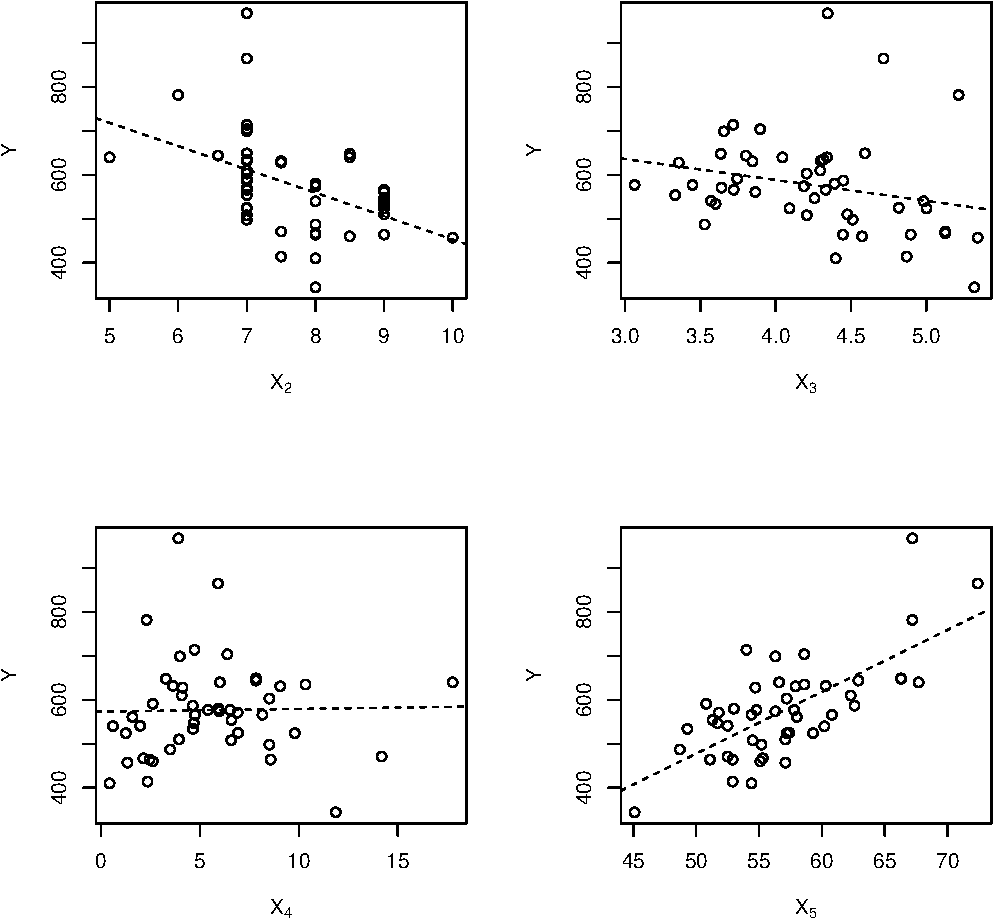
\includegraphics[width=0.49\linewidth]{finalexam_files/figure-latex/ex4-pairs-1} 

}

\caption{Plots of the response against covariates in the data.}\label{fig:ex4-pairs}
\end{figure}

\subsection{Part (b)}\label{part-b-3}

Start by fitting all the models. We also add a predictive function to the model:

\begin{Shaded}
\begin{Highlighting}[]
\CommentTok{\# model string}
\NormalTok{init\_model }\OtherTok{\textless{}{-}} \StringTok{"model\{}
\StringTok{  for (i in 1:n) \{}
\StringTok{    Y[i]  \textasciitilde{} dnorm(mu[i], tau)}
\StringTok{    Yp[i] \textasciitilde{} dnorm(mu[i], tau)}
\StringTok{    mu[i]   \textless{}{-} inprod(X[i,], beta)}
\StringTok{  \}}
\StringTok{  }
\StringTok{  for (j in 1:p) \{ beta[j] \textasciitilde{} dnorm(0, 0.0001)\}}
\StringTok{  }
\StringTok{  tau   \textasciitilde{} dgamma(0.1, 0.1)}
\StringTok{  sigma \textless{}{-} 1/tau}
\StringTok{\}"}

\CommentTok{\# construct model matrices for M1, ..., M4 on scaled data}
\NormalTok{X\_all }\OtherTok{\textless{}{-}} \FunctionTok{cbind}\NormalTok{(}\DecValTok{1}\NormalTok{, }\FunctionTok{scale}\NormalTok{(X2), }\FunctionTok{scale}\NormalTok{(X3), }\FunctionTok{scale}\NormalTok{(X4), }\FunctionTok{scale}\NormalTok{(X5))}
\NormalTok{X\_M1 }\OtherTok{\textless{}{-}}\NormalTok{ X\_all[,}\FunctionTok{c}\NormalTok{(}\DecValTok{1}\NormalTok{, }\DecValTok{3}\NormalTok{, }\DecValTok{5}\NormalTok{)]}
\NormalTok{X\_M2 }\OtherTok{\textless{}{-}}\NormalTok{ X\_all[,}\FunctionTok{c}\NormalTok{(}\DecValTok{1}\NormalTok{, }\DecValTok{2}\NormalTok{, }\DecValTok{3}\NormalTok{, }\DecValTok{5}\NormalTok{)]}
\NormalTok{X\_M3 }\OtherTok{\textless{}{-}}\NormalTok{ X\_all[,}\FunctionTok{c}\NormalTok{(}\DecValTok{1}\NormalTok{, }\DecValTok{3}\NormalTok{, }\DecValTok{4}\NormalTok{, }\DecValTok{5}\NormalTok{)]}
\NormalTok{X\_M4 }\OtherTok{\textless{}{-}}\NormalTok{ X\_all}

\CommentTok{\# create data vectors for fitting JAGS models}
\NormalTok{model\_matrices }\OtherTok{\textless{}{-}} \FunctionTok{list}\NormalTok{(X\_M1, X\_M2, X\_M3, X\_M4)}
\NormalTok{data\_vectors }\OtherTok{\textless{}{-}} \FunctionTok{lapply}\NormalTok{(}\DecValTok{1}\SpecialCharTok{:}\DecValTok{4}\NormalTok{, }\ControlFlowTok{function}\NormalTok{(i) \{}
\NormalTok{  X }\OtherTok{\textless{}{-}}\NormalTok{ model\_matrices[[i]] }\CommentTok{\# extract model matrix}
\NormalTok{  data }\OtherTok{\textless{}{-}} \FunctionTok{list}\NormalTok{(}\AttributeTok{X =}\NormalTok{ X, }\AttributeTok{Y =}\NormalTok{ Y, }\AttributeTok{n =} \FunctionTok{length}\NormalTok{(Y), }\AttributeTok{p =} \FunctionTok{ncol}\NormalTok{(X))}
\NormalTok{\})}

\NormalTok{jags\_models }\OtherTok{\textless{}{-}} \FunctionTok{lapply}\NormalTok{(data\_vectors, }\ControlFlowTok{function}\NormalTok{(data) \{}
\NormalTok{  model }\OtherTok{\textless{}{-}} \FunctionTok{jags.model}\NormalTok{(}\FunctionTok{textConnection}\NormalTok{(init\_model), data, }\AttributeTok{n.chains =} \DecValTok{4}\NormalTok{, }\AttributeTok{quiet =} \ConstantTok{TRUE}\NormalTok{)}
  \FunctionTok{update}\NormalTok{(model, }\AttributeTok{n.iter =} \DecValTok{3000}\NormalTok{, }\AttributeTok{progress.bar =} \StringTok{"none"}\NormalTok{)}
  \FunctionTok{return}\NormalTok{(model)}
\NormalTok{\})}
\end{Highlighting}
\end{Shaded}

The DICs are computed for the models below, shown in Table 4. Evidently, model \(\mathcal M_2\) is preferred.

\begin{Shaded}
\begin{Highlighting}[]
\NormalTok{jags\_dics }\OtherTok{\textless{}{-}} \FunctionTok{lapply}\NormalTok{(jags\_models, }\ControlFlowTok{function}\NormalTok{(model) \{}
  \FunctionTok{dic.samples}\NormalTok{(model, }\AttributeTok{n.iter =} \DecValTok{10000}\NormalTok{, }\AttributeTok{progress.bar =} \StringTok{"none"}\NormalTok{)}
\NormalTok{\})}
\NormalTok{jags\_dics}
\end{Highlighting}
\end{Shaded}

\begin{verbatim}
## [[1]]
## Mean deviance:  546.5 
## penalty 4.205 
## Penalized deviance: 550.7 
## 
## [[2]]
## Mean deviance:  539.7 
## penalty 5.215 
## Penalized deviance: 544.9 
## 
## [[3]]
## Mean deviance:  546.7 
## penalty 5.23 
## Penalized deviance: 551.9 
## 
## [[4]]
## Mean deviance:  540.3 
## penalty 6.254 
## Penalized deviance: 546.5
\end{verbatim}

\begin{table}[H]
  \centering
  \begin{tabular}{clrr}
    \toprule
    Model & Model form & DIC & $p_D$ \\
    \midrule
    $\mathcal M_1$ & $\mu_i = \beta_1 + X_{i3}\beta_3 + X_{i5}\beta_5$ & 550.69 & 4.21 \\
    $\mathcal M_2$ & $\mu_i = \beta_1 + X_{i2}\beta_2 + X_{i3}\beta_3 + X_{i5}\beta_5$ & 544.94 & 5.22 \\
    $\mathcal M_3$ & $\mu_i = \beta_1 + X_{i3}\beta_3 + X_{i4}\beta_4 + X_{i5}\beta_5$ & 551.89 & 5.23 \\
    $\mathcal M_4$ & $\mu_i = \beta_1 + X_{i2}\beta_2 + X_{i3}\beta_3 + X_{i4}\beta_4 + X_{i5}\beta_5$ & 546.53 & 6.25 \\
    \bottomrule
  \end{tabular}
  \caption{Model fit criteria for the linear models $\mathcal M_1, \ldots, \mathcal M_4$.}
  \label{ex4-table-dic}
\end{table}

\subsection{Part (c)}\label{part-c-3}

Based on the data in Table 4, the second model, \(\mathcal M_2\) is the one we will use. Therefore register it in a variable, before drawing some samples to summarise the posterior. Also, compute the residual vector \(\hat{\boldsymbol\varepsilon} = \mathbf y - \hat{\mathbf y}\).

\begin{Shaded}
\begin{Highlighting}[]
\NormalTok{model\_sel }\OtherTok{\textless{}{-}}\NormalTok{ jags\_models[[}\DecValTok{2}\NormalTok{]]}
\NormalTok{samples\_sel }\OtherTok{\textless{}{-}} \FunctionTok{coda.samples}\NormalTok{(model\_sel, }\AttributeTok{variable.names =} \FunctionTok{c}\NormalTok{(}\StringTok{"beta"}\NormalTok{, }\StringTok{"sigma"}\NormalTok{, }\StringTok{"Yp"}\NormalTok{), }
                            \AttributeTok{n.iter =} \DecValTok{10000}\NormalTok{, }\AttributeTok{progress.bar =} \StringTok{"none"}\NormalTok{)}

\NormalTok{Yp }\OtherTok{\textless{}{-}} \FunctionTok{summary}\NormalTok{(samples\_sel)}\SpecialCharTok{$}\NormalTok{statistics[}\DecValTok{1}\SpecialCharTok{:}\DecValTok{48}\NormalTok{, }\DecValTok{1}\NormalTok{]}
\NormalTok{resid }\OtherTok{\textless{}{-}}\NormalTok{ Y }\SpecialCharTok{{-}}\NormalTok{ Yp}
\end{Highlighting}
\end{Shaded}

Figure \ref{fig:ex4-resid-plots} below shows some diagnostic plots for the residuals. The structure of the residuals
in the index plot (left) is possibly non-linear and thus not distributed around zero (dashed line), as is indicated by the LOWESS line (red).
A normal Q-Q plot (middle) shows that the residuals stray quite a bit from the theoretical line, especially at the extremes. A histogram of the
residuals (right) shows that the distribution of residuals is quite right-skewed. These observations put together might indicate a problem with the model assumptions, namely that the residuals are zero-centred normal variables with constant variance.

\begin{figure}

{\centering 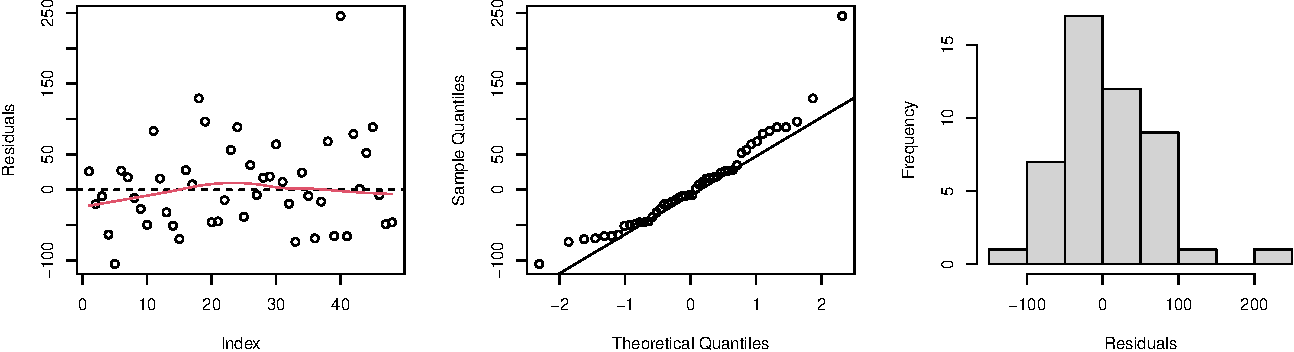
\includegraphics[width=1\linewidth]{finalexam_files/figure-latex/ex4-resid-plots-1} 

}

\caption{Residual plots for the DIC optimal model, $\mathcal M_2$.}\label{fig:ex4-resid-plots}
\end{figure}

\subsection{Part (d)}\label{part-d-1}

The requested plots are shown below in Figures \ref{fig:ex4-resids-vs-cov} and \ref{fig:ex4-resids-vs-fit}. When plotted against \(X_2\), there is possible indication of non-constant variance and non-linearity in residuals.
Additionally, the structure in the plot to the right (\(X_5\)) indicates non-linearity. The middle plot (\(X_3\)) is a bit more vague. We can not say for certain that the expectation of the residuals as a function of \(X_2\) and \(X_5\) is zero, which is problematic. Figure \ref{fig:ex4-resids-vs-fit} also seems to indicate that the residual structure is normally distributed around zero, and it is not clear whether variance is constant. However it also shows that the model seems to predict fairly well, so we use it.

\begin{figure}

{\centering 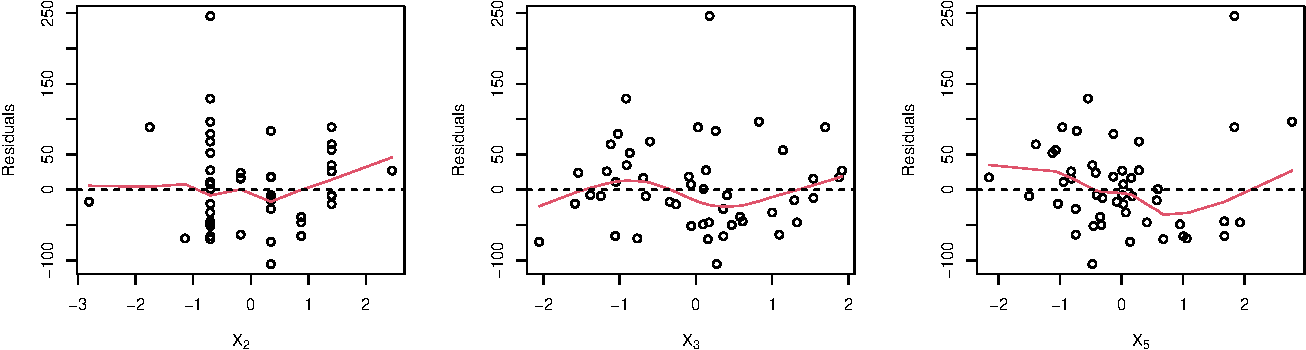
\includegraphics[width=1\linewidth]{finalexam_files/figure-latex/ex4-resids-vs-cov-1} 

}

\caption{Residuals against each of the covariates in model $\mathcal M_2$.}\label{fig:ex4-resids-vs-cov}
\end{figure}

\begin{figure}

{\centering 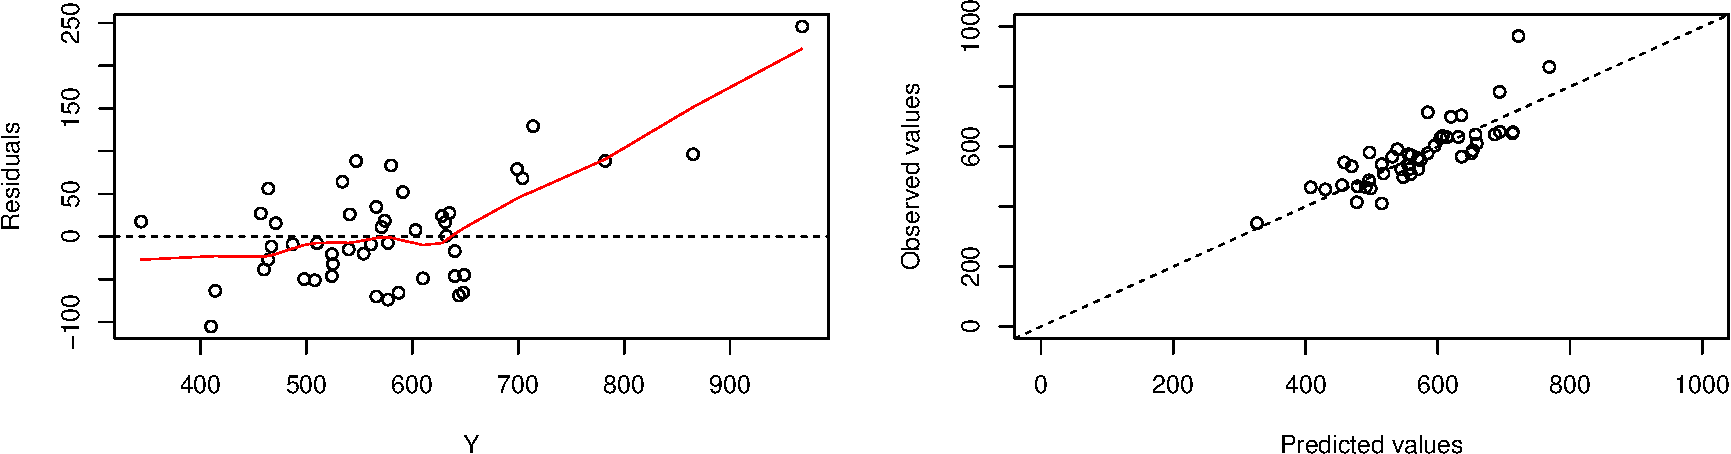
\includegraphics[width=1\linewidth]{finalexam_files/figure-latex/ex4-resids-vs-fit-1} 

}

\caption{Residuals against fitted values in model $\mathcal M_2$ (left), observed versus fitted values (right).}\label{fig:ex4-resids-vs-fit}
\end{figure}

\subsection{Part (e)}\label{part-e-1}

Here is a summary of the samples, trimmed to only display the relevant parameters:

\begin{Shaded}
\begin{Highlighting}[]
\NormalTok{sum\_samples\_sel }\OtherTok{\textless{}{-}} \FunctionTok{summary}\NormalTok{(samples\_sel); sum\_samples\_sel}
\end{Highlighting}
\end{Shaded}

\begin{verbatim}
## 
## Iterations = 13001:23000
## Thinning interval = 1
## Number of chains = 4
## Sample size per chain = 10000
## 
## 1. Empirical mean and standard deviation for each variable,
##    plus standard error of the mean:
\end{verbatim}

\begin{verbatim}
##               Mean          SD   Naive SE Time-series SE
## beta[1]  571.33255    9.714891 0.04857446     0.04958464
## beta[2]  -27.90382   10.238787 0.05119393     0.05575517
## beta[3]  -38.51123    9.938218 0.04969109     0.05087810
## beta[4]   75.57987   10.346895 0.05173447     0.05819385
## sigma   4550.36786 1018.409355 5.09204677     5.57017845
\end{verbatim}

\begin{verbatim}
## 
## 2. Quantiles for each variable:
\end{verbatim}

\begin{verbatim}
##               2.5%        25%        50%        75%      97.5%
## beta[1]  551.77878  564.90555  571.50234  577.86255  590.18644
## beta[2]  -48.04657  -34.71973  -27.94898  -21.05806   -7.75176
## beta[3]  -58.27586  -45.07145  -38.50538  -31.96702  -18.94362
## beta[4]   54.92778   68.79402   75.58126   82.46751   95.95370
## sigma   2980.10463 3829.89212 4409.98354 5108.85005 6961.06665
\end{verbatim}

These are also shown in Table 5 below:

\begin{table}[H]
  \centering
  \begin{tabular}{clll}
    \toprule
          & Mean & Standard deviation & 95\% credible set \\
    \midrule
    $\beta_1$      & 571.3325501 & 9.7148912 & $[551.7787761, 590.1864427]$ \\
    $\beta_2$      & -27.9038219 & 10.238787 & $[-48.0465686, -7.7517599]$ \\
    $\beta_3$      & -38.51123 & 9.9382177 & $[-58.2758558, -18.9436242]$ \\
    $\beta_5$      & 75.5798728 & 10.3468949 & $[54.9277794, 95.9537027]$ \\
    $\sigma^2$     & 4550.3678643 & 1018.4093545 & $[2980.1046342, 6961.0666507]$ \\
    \bottomrule
  \end{tabular}
  \label{tab:ex2-sum-stats-lin}
  \caption{Summary statistics for the coefficients in the linear model $\mathcal M_2$.}
\end{table}

\subsection{Part (f)}\label{part-f-1}

We will use Table 5 for this purpose. We see that the intercept coefficient is \(\beta_1 = 571.33\), which tells us that if all the other scaled covariates were set to zero, the consumption of petrol would be \(571.33\) millions of gallons. We must take some care in interpreting the coefficients in the normal units because we scaled the data when performing Bayesian linear regression. Due to the nature of scaling, a unit increase in standard unit corresponds to a unit standard deviation increment in the original covariate.

Credible sets follow directly from the ones presented in the table. For \(X_2\), the coefficient is \(\beta_2 = -27.9\), which means that increasing the petrol tax by one standard deviation would result in a decrease of approximately \(-27.9\) millions of gallons of petrol consumption per year (which may seem contradictory, but the relationship is reinforced in the data). Increasing the covariate \(X_3\) by one standard deviation, or the per capita income by a thousand dollars, results in a decrease of \(-38.51\) millions of gallons of petrol consumption per year. A unit standard deviation increase in \(X_5\) (percentage of population with drivers license) causes fuel consumption to increase by \(\beta_5 = 75.58\) millions of gallons.

\subsection{Part (g)}\label{part-g-1}

Set up a new \textsf{JAGS} model below, one which predicts the fuel consumption for the unobserved data. We will have to redefine the model matrix to include the unobserved data and scale it, before separating the two. Summarising the data following the fit will allow us to verify that this does not affect the model fit.

\begin{Shaded}
\begin{Highlighting}[]
\NormalTok{X\_M2\_unobs }\OtherTok{\textless{}{-}} \FunctionTok{rbind}\NormalTok{(}\FunctionTok{cbind}\NormalTok{(}\DecValTok{1}\NormalTok{, X2, X3, X5), }\FunctionTok{c}\NormalTok{(}\DecValTok{1}\NormalTok{, }\DecValTok{7}\NormalTok{, }\FloatTok{3.300}\NormalTok{, }\DecValTok{51}\NormalTok{))}
\NormalTok{X\_M2\_unobs[,}\DecValTok{2}\NormalTok{] }\OtherTok{\textless{}{-}} \FunctionTok{scale}\NormalTok{(X\_M2\_unobs[,}\DecValTok{2}\NormalTok{])}
\NormalTok{X\_M2\_unobs[,}\DecValTok{3}\NormalTok{] }\OtherTok{\textless{}{-}} \FunctionTok{scale}\NormalTok{(X\_M2\_unobs[,}\DecValTok{3}\NormalTok{])}
\NormalTok{X\_M2\_unobs[,}\DecValTok{4}\NormalTok{] }\OtherTok{\textless{}{-}} \FunctionTok{scale}\NormalTok{(X\_M2\_unobs[,}\DecValTok{4}\NormalTok{])}

\NormalTok{X\_pr       }\OtherTok{\textless{}{-}}\NormalTok{ X\_M2\_unobs[}\DecValTok{49}\NormalTok{,]}
\NormalTok{X\_M2\_unobs }\OtherTok{\textless{}{-}}\NormalTok{ X\_M2\_unobs[}\SpecialCharTok{{-}}\DecValTok{49}\NormalTok{,]}

\NormalTok{init\_model }\OtherTok{\textless{}{-}} \FunctionTok{textConnection}\NormalTok{(}\StringTok{"model\{}
\StringTok{  for (i in 1:n) \{}
\StringTok{    Y[i]  \textasciitilde{} dnorm(mu[i], tau)}
\StringTok{    mu[i]   \textless{}{-} inprod(X[i,], beta)}
\StringTok{  \}}
\StringTok{  }
\StringTok{  Y\_pr \textasciitilde{} dnorm(inprod(X\_pr, beta), tau)}
\StringTok{  }
\StringTok{  for (j in 1:p) \{ beta[j] \textasciitilde{} dnorm(0, 0.0001)\}}
\StringTok{  }
\StringTok{  tau   \textasciitilde{} dgamma(0.1, 0.1)}
\StringTok{  sigma \textless{}{-} 1/tau}
\StringTok{\}"}\NormalTok{)}

\NormalTok{data }\OtherTok{\textless{}{-}} \FunctionTok{list}\NormalTok{(}\AttributeTok{X =}\NormalTok{ X\_M2, }\AttributeTok{Y =}\NormalTok{ Y, }\AttributeTok{X\_pr =}\NormalTok{ X\_pr, }\AttributeTok{n =} \FunctionTok{nrow}\NormalTok{(X\_M2), }\AttributeTok{p =} \FunctionTok{ncol}\NormalTok{(X\_M2))}

\NormalTok{model\_ppd }\OtherTok{\textless{}{-}} \FunctionTok{jags.model}\NormalTok{(init\_model, }\AttributeTok{data =}\NormalTok{ data, }\AttributeTok{n.chains =} \DecValTok{2}\NormalTok{, }\AttributeTok{quiet =} \ConstantTok{TRUE}\NormalTok{)}
\FunctionTok{update}\NormalTok{(model\_ppd, }\AttributeTok{n.iter =} \DecValTok{3000}\NormalTok{, }\AttributeTok{progress.bar =} \StringTok{"none"}\NormalTok{)}

\NormalTok{samples\_ppd }\OtherTok{\textless{}{-}} \FunctionTok{coda.samples}\NormalTok{(model\_ppd, }\AttributeTok{variable.names =} \FunctionTok{c}\NormalTok{(}\StringTok{"beta"}\NormalTok{, }\StringTok{"sigma"}\NormalTok{, }\StringTok{"Y\_pr"}\NormalTok{), }
                            \AttributeTok{n.iter =} \DecValTok{10000}\NormalTok{, }\AttributeTok{progress.bar =} \StringTok{"none"}\NormalTok{)}
\end{Highlighting}
\end{Shaded}

Summarise the posterior:

\begin{Shaded}
\begin{Highlighting}[]
\NormalTok{sum\_ppd }\OtherTok{\textless{}{-}} \FunctionTok{summary}\NormalTok{(samples\_ppd)}
\NormalTok{sum\_ppd}
\end{Highlighting}
\end{Shaded}

\begin{verbatim}
## 
## Iterations = 3001:13000
## Thinning interval = 1 
## Number of chains = 2 
## Sample size per chain = 10000 
## 
## 1. Empirical mean and standard deviation for each variable,
##    plus standard error of the mean:
## 
##            Mean       SD Naive SE Time-series SE
## Y_pr     571.44   71.009  0.50211        0.50210
## beta[1]  571.25    9.752  0.06896        0.06896
## beta[2]  -27.89   10.267  0.07260        0.07947
## beta[3]  -38.58    9.895  0.06996        0.07131
## beta[4]   75.51   10.399  0.07354        0.08136
## sigma   4569.19 1027.699  7.26693        7.99668
## 
## 2. Quantiles for each variable:
## 
##            2.5%     25%     50%     75%   97.5%
## Y_pr     429.37  525.00  572.15  618.41  709.81
## beta[1]  551.69  564.84  571.45  577.79  590.00
## beta[2]  -47.88  -34.66  -28.05  -21.08   -7.46
## beta[3]  -57.82  -45.17  -38.69  -32.02  -18.95
## beta[4]   55.07   68.61   75.57   82.38   95.74
## sigma   2984.43 3836.40 4429.08 5144.49 6938.48
\end{verbatim}

The estimates of the linear regression seem to be unchanged by our wrangling of the data, which is good. The mean of the posterior predictive distribution is 571.44 with 95\% credible interval \([429.37, 709.81]\).
A density plot of the samples drawn from the PPD of the unobserved data is shown in \ref{fig:ex4-fig-density} below.

\begin{figure}

{\centering 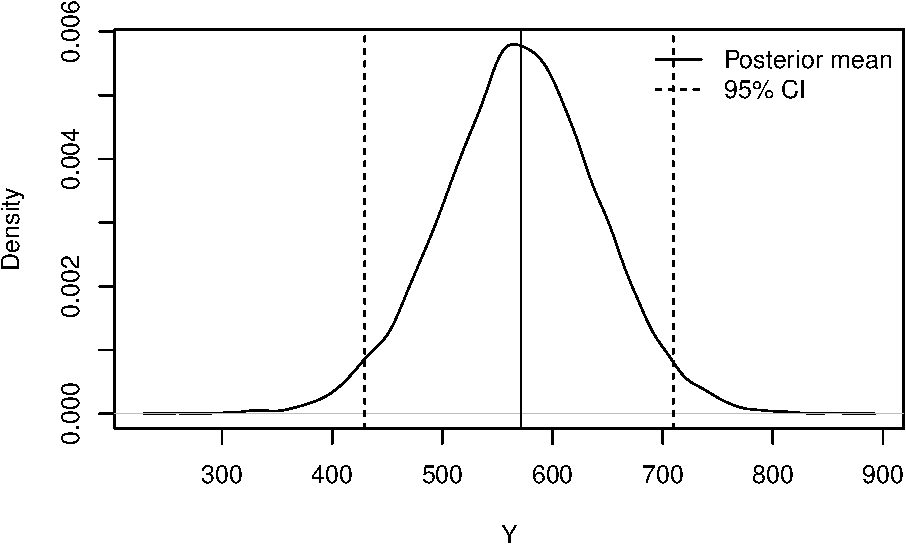
\includegraphics[width=0.75\linewidth]{finalexam_files/figure-latex/ex4-fig-density-1} 

}

\caption{Density plot of samples for the posterior predictive distribution of the unobserved data.}\label{fig:ex4-fig-density}
\end{figure}

\newpage

\section{Exercise 5}\label{exercise-5}

The data in the file \texttt{problem5.txt} contain the height of 26 boys living in Oxford in England over a two year period. Each boy is measured on nine different occasions over a period
of two years. The first column contains the identity number of each boy, the second column contains the time variable (in years, starts at \(-1.0\), ends at a number close to \(1.0\))
and the third column contains the height of the boys at the specified time point. The table below illustrates the form of the data.

\begin{table}[H]
  \centering
  \begin{tabular}{lcc}
    \toprule
    id & time & height \\
    \midrule
    Boy 1  & -1.0000 & 140.52 \\
    Boy 2  & -0.7479 & 143.42 \\
    \vdots &  \vdots & \vdots \\
    Boy 1  &  0.9945& 155.89 \\
    Boy 2  & -1.0000 & 136.91 \\
    \vdots &  \vdots & \vdots \\
    Boy 2  &  0.9945 & 148.39 \\
    \vdots &  \vdots & \vdots \\
    \bottomrule
  \end{tabular}
\end{table}

Let \(Y_{ij}\) be the height of the \(i\)th boy at time \(X_{ij}\) (the \(j\)th time point for the \(i\)th boy). It is assumed that the height increase linearly with time for each boy. However, the growth may vary between boys. Thus, the following model is proposed
\[
  Y_{ij} = \alpha_{i1} + \alpha_{i2} X_{ij} + \varepsilon_{ij}, \quad \varepsilon_{ij} \sim \mathcal N(0, \sigma^2),
\]
\(j = 1, \ldots, T\), \(i = 1, \ldots, n\) where \(T\) is the number of measurements taken of each boy \(i\) (\(T = 9\)), and \(n\) is the number of boys (\(n = 26\)). Here \(\varepsilon_{ij}\) is the
mean-zero deviation of the \(j\)th measurement from the linear model for the \(i\)th boy and \(\sigma^2\) is its variance. It is assumed that the \(\varepsilon_{ij}\)s are independent of each
other.

Each \(\boldsymbol\alpha_i = (\alpha_{i1}, \alpha_{i2})^\intercal\) is assigned a bivariate Gaussian distribution with mean \(\boldsymbol\beta\) and covariance matrix \(\boldsymbol\Omega\),
that is,
\[
  \boldsymbol\alpha_i \sim \mathcal N(\boldsymbol\beta, \boldsymbol\Omega), \quad i \in \{1, \ldots, n\}.
\]

The following prior distributions are assigned to \(\sigma^2\), \(\boldsymbol\beta\) and \(\boldsymbol\Omega\),
\begin{align*}
  &\sigma^2 \sim \mathrm{InvGamma}(0.1, 0.1), \\
  &\boldsymbol\beta \sim \mathcal N(\mathbf 0, 100^2\mathbf I_2), \\
  &\boldsymbol\Omega \sim \mathrm{InvWishart}(2.1, \mathbf I/ 2.1).
\end{align*}

\begin{enumerate}[label = (\alph*)]
  \item Find the posterior distribution of the unknown parameters in the hierarchical model. Present it in terms of the densities of the $Y_{ij}$s, the $\boldsymbol\alpha_i$s,
  $\sigma^2$, $\boldsymbol\beta$ and $\boldsymbol\Omega$.
  
  \item Specify the data layer, the process layer and the prior layer of the hierarchical model, that is, specify which variables/parameters are modeled at each layer, and what         
  probability models are assumed at each level.
  
  \item Write code in \textsf{JAGS} within \textsf{R} to sample from the posterior density of the unknown parameters, and present the code. If another programming language than \textsf{R} (with \textsf{JAGS}) is used,
  please present the code that you use to sample from the posterior density of the unknown parameters.
  
  \item Compute the posterior means and 95\% posterior intervals for $\alpha_{11}, \ldots, \alpha_{n1}, \alpha_{12}, \ldots, \alpha_{n2}, \sigma^2, \boldsymbol\beta$ and $\boldsymbol\Omega$. Use four chains where each chain consists of 13000 iterations and the first 3000 are used for burn-in. Present the $\alpha_{i1}$s and the $\alpha_{i2}$s
  in two separate figures, that is, plot the id-number of the boys on the $x$-axis and the 95\% posterior intervals along with a point for the posterior mean on the $y$-axis.
  Present $\sigma^2$, $\boldsymbol\beta$ and $\boldsymbol\Omega$ in a table.
  
  \item For each of the 26 boys plot as dots the observed heights on the $y$-axis and corresponding times on the $x$-axis. This gives 26 figures. These figures can, for example, be arranged in a seven by four matrix (with two spots empty). In the case of the plot for the $i$th boy, draw a line based on the formula $\alpha_{i1} + \alpha_{i2}x$ where $x$
  goes from $-1.1$ to $1.1$. Use the posterior means of $\alpha_{i1}$ and $\alpha_{i2}$. Does the model appear to fit the data adequately well?
\end{enumerate}

\section{Solution}\label{solution-4}

\subsection{Part (a)}\label{part-a-4}

The joint posterior distribution of the unobserved variables \(\boldsymbol\alpha_1, \ldots, \boldsymbol\alpha_n, \boldsymbol\beta, \boldsymbol\Omega, \sigma^2\) can be decomposed as follows:

\[
p(\boldsymbol\alpha_1, \ldots, \boldsymbol\alpha_n, \boldsymbol\beta, \boldsymbol\Omega, \sigma^2 | \mathbf Y)
\propto \mathcal L(\mathbf Y | \boldsymbol\alpha_1, \ldots, \boldsymbol\alpha_n, \sigma^2) \pi(\boldsymbol\alpha_1, \ldots, \boldsymbol\alpha_n | \boldsymbol\beta, \boldsymbol\Omega) \pi(\boldsymbol\beta)\pi(\boldsymbol\Omega)\pi(\sigma^2)
\]
To see why this is true, it helps to look at Figure \ref{fig:ex5-dag-representation} and trace through the dependencies for the \(\mathbf Y_i\)s. Now,
\begin{align*}
p(\boldsymbol\alpha_1, \ldots, \boldsymbol\alpha_n, \boldsymbol\beta, \boldsymbol\Omega, \sigma^2 | \mathbf Y)
&\propto \prod_{i = 1}^n \left[ \prod_{j = 1}^T \mathcal L(\mathbf Y_i | \boldsymbol\alpha_i, \sigma^2) \pi(\boldsymbol\alpha_i | \boldsymbol\beta, \boldsymbol\Omega) \right] \pi(\boldsymbol\beta) \pi(\boldsymbol\Omega) \pi(\sigma^2) \\
&\propto \prod_{i = 1}^n \left[\prod_{j = 1}^T (\sigma^2)^{-1/2} \exp\left(\frac{(Y_{ij} - \alpha_{i1} - \alpha_{i2}X_{ij})^2}{2\sigma^2}\right)\right] |\boldsymbol\Omega|^{-1/2} \cdots \\
&\hphantom{\propto} \exp\left(- \frac{1}{2} (\boldsymbol\alpha_i - \boldsymbol\beta)^\intercal \boldsymbol\Omega^{-1} (\boldsymbol\alpha_i - \boldsymbol\beta)\right) (\sigma^2)^{- a - 1} \exp[-b/\sigma^2] \cdots \\
&\hphantom{\propto} \exp\left(- \frac{1}{2} \boldsymbol\beta^\intercal (m^2 \mathbf I_2)^{-1} \boldsymbol\beta\right) |\boldsymbol\Omega|^{-(p - \nu - 1)/2} \exp \left[- \frac{1}{2} \tr\left(\frac{\mathbf I_2}{\nu} \boldsymbol\Omega^{-1}\right)\right] \\
&= (\sigma^2)^{-nT/2 - a - 1} |\boldsymbol\Omega|^{-(n + p - \nu - 1)/2} \exp\Biggr[- \frac{1}{2} \Biggl(\frac{\sum_{i = 1}^n \sum_{j = 1}^T (Y_{ij} - \alpha_{i1} - \alpha_{i2} X_{ij})^2}{\sigma^2}\cdots \\
&\hphantom{=} \cdots + \frac{2b}{\sigma^2} + (\boldsymbol\alpha_i - \boldsymbol\beta)^\intercal \boldsymbol\Omega(\boldsymbol\alpha_i - \boldsymbol\beta) + \frac{1}{m^2} \boldsymbol\beta^\intercal \boldsymbol\beta + \tr\left(\frac{1}{\nu} \boldsymbol\Omega^{-1} \right)\Biggl)\Biggr],
\end{align*}

where \(a = b = 0.1\), \(\nu = 2.1\), \(p = 2\) and \(m = 100\).

\subsection{Part (b)}\label{part-b-4}

Figure \ref{fig:ex5-dag-representation} shows the DAG representation of the model. The lowest nodes represent the data layer, where we have \(\boldsymbol\beta \sim \mathcal N(\mathbf 0, 100^2 \mathbf I)\) which
is can be thought of as the vector which fixes the centre of the distribution of growth curves for the boys. The other matrix parameter \(\boldsymbol\Omega \sim \mathrm{InvWishart}(2.1, \mathbf I/2.1)\) is used to control the spread of the growth curves, and together they feed into the growth curve parameters for the \(i\)th boy, \(\boldsymbol\alpha_i\). Here the assumption is made that these two parameters can give a reasonable range for each of the growth curves which will then be used to model the data. The parameter \(\sigma^2\) controls the variation of the observed height around the linear predictor \(\alpha_{i1} + \alpha_{i2}X_{ij}\). This parameter feeds into the nodes \(\mathbf Y_1, \ldots, \mathbf Y_n\), where \(\mathbf Y_i = (Y_{i1}, \ldots, Y_{iT})\).

The process layer is in the middle and consists of the \(\boldsymbol\alpha_i\)s. This is where the latent data generating mechanism is constructed, i.e.~the growth curves for each of the boys, \(\boldsymbol\alpha_i = (\alpha_{i1}, \alpha_{i2})^\intercal\). These are multivariate normal random variables with centre \(\boldsymbol\beta\) and spread \(\boldsymbol\Omega\), that is \(\boldsymbol\alpha_i \sim \mathcal N(\boldsymbol\beta, \boldsymbol\Omega)\). The assumption made here is that each of the growth curves stems from the same distributions, i.e.~that they are independent and identically distributed.

Lastly, the data layer is shown at the top. Here we have nodes \(\mathbf Y_1, \ldots, \mathbf Y_n\), one for each boy, consisting of their height measurements. Here, \(Y_{ij} \sim \mathcal N\left(\alpha_{i1} + \alpha_{i2} X _{ij}, \sigma^2\right)\) for each \(j \in \{1, \ldots, T\}\), assuming that a linear regression model is appropriate for these data.

\begin{figure}[H]
\centering
\begin{tikzpicture}
\begin{scope}[every node/.style={circle,thick,draw}]
    \node (D1) at (0,0) {$\mathbf Y_1$};
    \node (D2) at (1,0) {$\mathbf Y_2$};
    \node (D3) at (3,0) {$\mathbf Y_n$};
    \node (P1) at (0,-1.5) {$\boldsymbol\alpha_1$};
    \node (P2) at (1,-1.5) {$\boldsymbol\alpha_2$};
    \node (P3) at (3,-1.5) {$\boldsymbol\alpha_n$};
    \node (p1) at (0.5,-3.0) {$\boldsymbol\beta$};
    \node (p2) at (1.5,-3.0) {$\boldsymbol\Omega$};
    \node (p3) at (2.5,-3.0) {$\sigma^2$};
\end{scope}

\begin{scope}[>={Stealth[black]},
              every node/.style={fill=white,circle},
              every edge/.style={draw}]
    \path [->] (p1) edge (P1);
    \path [->] (p1) edge (P2);
    \path [->] (p1) edge (P3);
    \path [->] (p2) edge (P1);
    \path [->] (p2) edge (P2);
    \path [->] (p2) edge (P3);
    \path [->] (P1) edge (D1);
    \path [->] (P2) edge (D2);
    \path [->] (P3) edge (D3);
\end{scope}

\draw (3.0, -3.0) -| (4, -0.85);
\draw (4, -0.85) -- (0, -0.85);


\node at (2,0) {$\ldots$};
\node at (2,-1.5) {$\ldots$};

\end{tikzpicture}
\caption{A DAG representation of the model.}
\label{fig:ex5-dag-representation}
\end{figure}

\subsection{Part (c)}\label{part-c-4}

Start by importing the data:

\begin{Shaded}
\begin{Highlighting}[]
\NormalTok{data5  }\OtherTok{\textless{}{-}} \FunctionTok{read.table}\NormalTok{(}\StringTok{"data/problem5.txt"}\NormalTok{, }\AttributeTok{header=}\ConstantTok{TRUE}\NormalTok{)}
\NormalTok{id     }\OtherTok{\textless{}{-}}\NormalTok{ data5[,}\DecValTok{1}\NormalTok{] }
\NormalTok{time   }\OtherTok{\textless{}{-}}\NormalTok{ data5[,}\DecValTok{2}\NormalTok{]}
\NormalTok{height }\OtherTok{\textless{}{-}}\NormalTok{ data5[,}\DecValTok{3}\NormalTok{]}

\NormalTok{T }\OtherTok{\textless{}{-}} \DecValTok{9}\NormalTok{; n }\OtherTok{\textless{}{-}} \DecValTok{26}

\NormalTok{X }\OtherTok{\textless{}{-}} \FunctionTok{matrix}\NormalTok{(}\AttributeTok{nrow =}\NormalTok{ n, }\AttributeTok{ncol =}\NormalTok{ T)}
\NormalTok{Y }\OtherTok{\textless{}{-}} \FunctionTok{matrix}\NormalTok{(}\AttributeTok{nrow =}\NormalTok{ n, }\AttributeTok{ncol =}\NormalTok{ T)}

\ControlFlowTok{for}\NormalTok{(i }\ControlFlowTok{in} \DecValTok{1}\SpecialCharTok{:}\NormalTok{n)\{}
  \ControlFlowTok{for}\NormalTok{(j }\ControlFlowTok{in} \DecValTok{1}\SpecialCharTok{:}\NormalTok{T)\{}
\NormalTok{    k }\OtherTok{\textless{}{-}}\NormalTok{ j }\SpecialCharTok{+}\NormalTok{ T}\SpecialCharTok{*}\NormalTok{(i }\SpecialCharTok{{-}} \DecValTok{1}\NormalTok{)}
\NormalTok{    X[i,j] }\OtherTok{\textless{}{-}}\NormalTok{ time[k]  }
\NormalTok{    Y[i,j] }\OtherTok{\textless{}{-}}\NormalTok{ height[k]}
\NormalTok{  \} \}}

\NormalTok{data }\OtherTok{\textless{}{-}} \FunctionTok{list}\NormalTok{(}\AttributeTok{X =}\NormalTok{ X, }\AttributeTok{Y =}\NormalTok{ Y, }\AttributeTok{n =}\NormalTok{ n, }\AttributeTok{T =}\NormalTok{ T)}
\end{Highlighting}
\end{Shaded}

Now fit the model in \textsf{JAGS}:

\begin{Shaded}
\begin{Highlighting}[]
\NormalTok{init\_height }\OtherTok{\textless{}{-}} \FunctionTok{textConnection}\NormalTok{(}\StringTok{"model\{}
\StringTok{  for (i in 1:n) \{}
\StringTok{    for(j in 1:T) \{}
\StringTok{      Y[i, j] \textasciitilde{} dnorm(alpha[i, 1] + alpha[i, 2] * X[i, j], tau)}
\StringTok{  \} \}}
\StringTok{    }
\StringTok{  for (i in 1:n) \{ alpha[i, 1:2] \textasciitilde{} dmnorm(beta[1:2], Omega[1:2, 1:2]) \}}
\StringTok{  }
\StringTok{  for (i in 1:2) \{ beta[i] \textasciitilde{} dnorm(0, 0.0001) \}}
\StringTok{  }
\StringTok{  tau \textasciitilde{} dgamma(0.1, 0.1)}
\StringTok{  }
\StringTok{  Omega[1:2,1:2] \textasciitilde{} dwish(R[,],2.1)}

\StringTok{  R[1,1]\textless{}{-}1/2.1}
\StringTok{  R[1,2]\textless{}{-}0}
\StringTok{  R[2,1]\textless{}{-}0}
\StringTok{  R[2,2]\textless{}{-}1/2.1}
\StringTok{  }
\StringTok{  sigma \textless{}{-} 1/tau}
\StringTok{\}"}\NormalTok{)}

\NormalTok{params  }\OtherTok{\textless{}{-}} \FunctionTok{c}\NormalTok{(}\StringTok{"beta"}\NormalTok{,}\StringTok{"alpha"}\NormalTok{,}\StringTok{"sigma"}\NormalTok{,}\StringTok{"Omega"}\NormalTok{)}
\NormalTok{model   }\OtherTok{\textless{}{-}} \FunctionTok{jags.model}\NormalTok{(init\_height, }\AttributeTok{data =}\NormalTok{ data, }\AttributeTok{n.chains =} \DecValTok{4}\NormalTok{, }\AttributeTok{quiet=}\ConstantTok{TRUE}\NormalTok{)}
\FunctionTok{update}\NormalTok{(model, }\DecValTok{3000}\NormalTok{, }\AttributeTok{progress.bar=}\StringTok{"none"}\NormalTok{)}
\NormalTok{samples\_height }\OtherTok{\textless{}{-}} \FunctionTok{coda.samples}\NormalTok{(model, }\AttributeTok{variable.names =}\NormalTok{ params, }\AttributeTok{n.iter =} \DecValTok{10000}\NormalTok{, }
                               \AttributeTok{progress.bar=}\StringTok{"none"}\NormalTok{)}
\end{Highlighting}
\end{Shaded}

\subsection{Part (d)}\label{part-d-2}

We will use the samples generated in (c) to summarise the posterior. Firstly, compute the
summary:

\begin{Shaded}
\begin{Highlighting}[]
\NormalTok{sum\_samples\_height }\OtherTok{\textless{}{-}} \FunctionTok{summary}\NormalTok{(samples\_height)}
\end{Highlighting}
\end{Shaded}

Figure \ref{fig:ex5-fig-post-mean-heights} shows a plot of the posterior means of model parameters \(\alpha_{11}, \ldots, \alpha_{n1}\) and \(\alpha_{12}, \ldots, \alpha_{n2}\).

\begin{figure}

{\centering 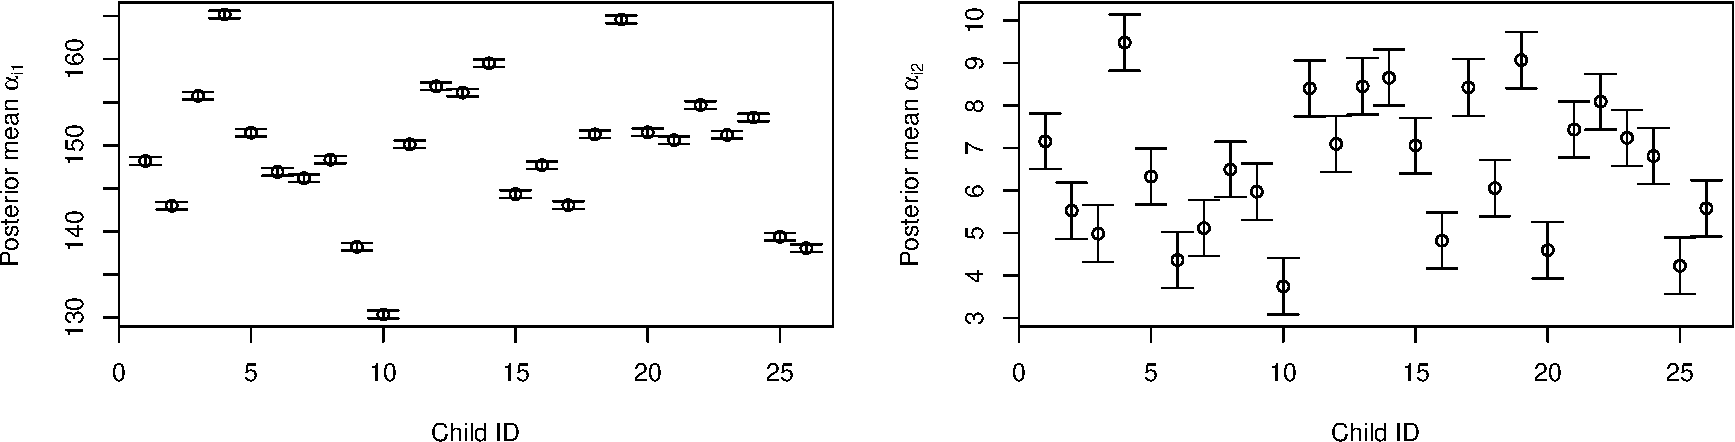
\includegraphics[width=1\linewidth]{finalexam_files/figure-latex/ex5-fig-post-mean-heights-1} 

}

\caption{Posterior means of $\alpha_{i1}$ and $\alpha_{i2}$ for the children along with 95\% credible sets.}\label{fig:ex5-fig-post-mean-heights}
\end{figure}

\begin{table}[H]
  \centering
  \begin{tabular}{clll}
    \toprule
          & Mean & 95\% credible set \\
    \midrule
    $\sigma^2$      & 0.455153 & $[0.369989, 0.5582852]$ \\
    $\boldsymbol\beta$ & $\begin{pmatrix}149.4005434 \\ 6.578375\end{pmatrix}$ & $\left[\begin{pmatrix}146.2616937 \\ 5.9049372\end{pmatrix}, 
       \begin{pmatrix}152.528671 \\ 7.2403505\end{pmatrix}\right]$ \\
    $\boldsymbol\Omega$ & $\begin{pmatrix}0.0288314 & -0.0907949 \\
                                          -0.0907949 & 0.6785469\end{pmatrix}$
                        & $\left[
                            \begin{pmatrix}0.0152466 & -0.1681471 \\
                                           -0.1681471 & 0.3490058\end{pmatrix},
                            \begin{pmatrix}0.0469607 & -0.0338223 \\
                                           -0.0338223 & 1.1430574\end{pmatrix}
                          \right]$ \\
    \bottomrule
  \end{tabular}
  \label{tab:ex5-sum-stats}
  \caption{Summary statistics for the coefficients in the linear model $\mathcal M_2$.}
\end{table}

\subsection{Part (e)}\label{part-e-2}

Figure \ref{fig:ex5-final-fig} shows observed height measurements for each of the boys as a function of time as dots connected by dashed lines.
The red line is the predicted change in height over time. As can be seen, the model appears to fit the data quite well.

\begin{figure}

{\centering 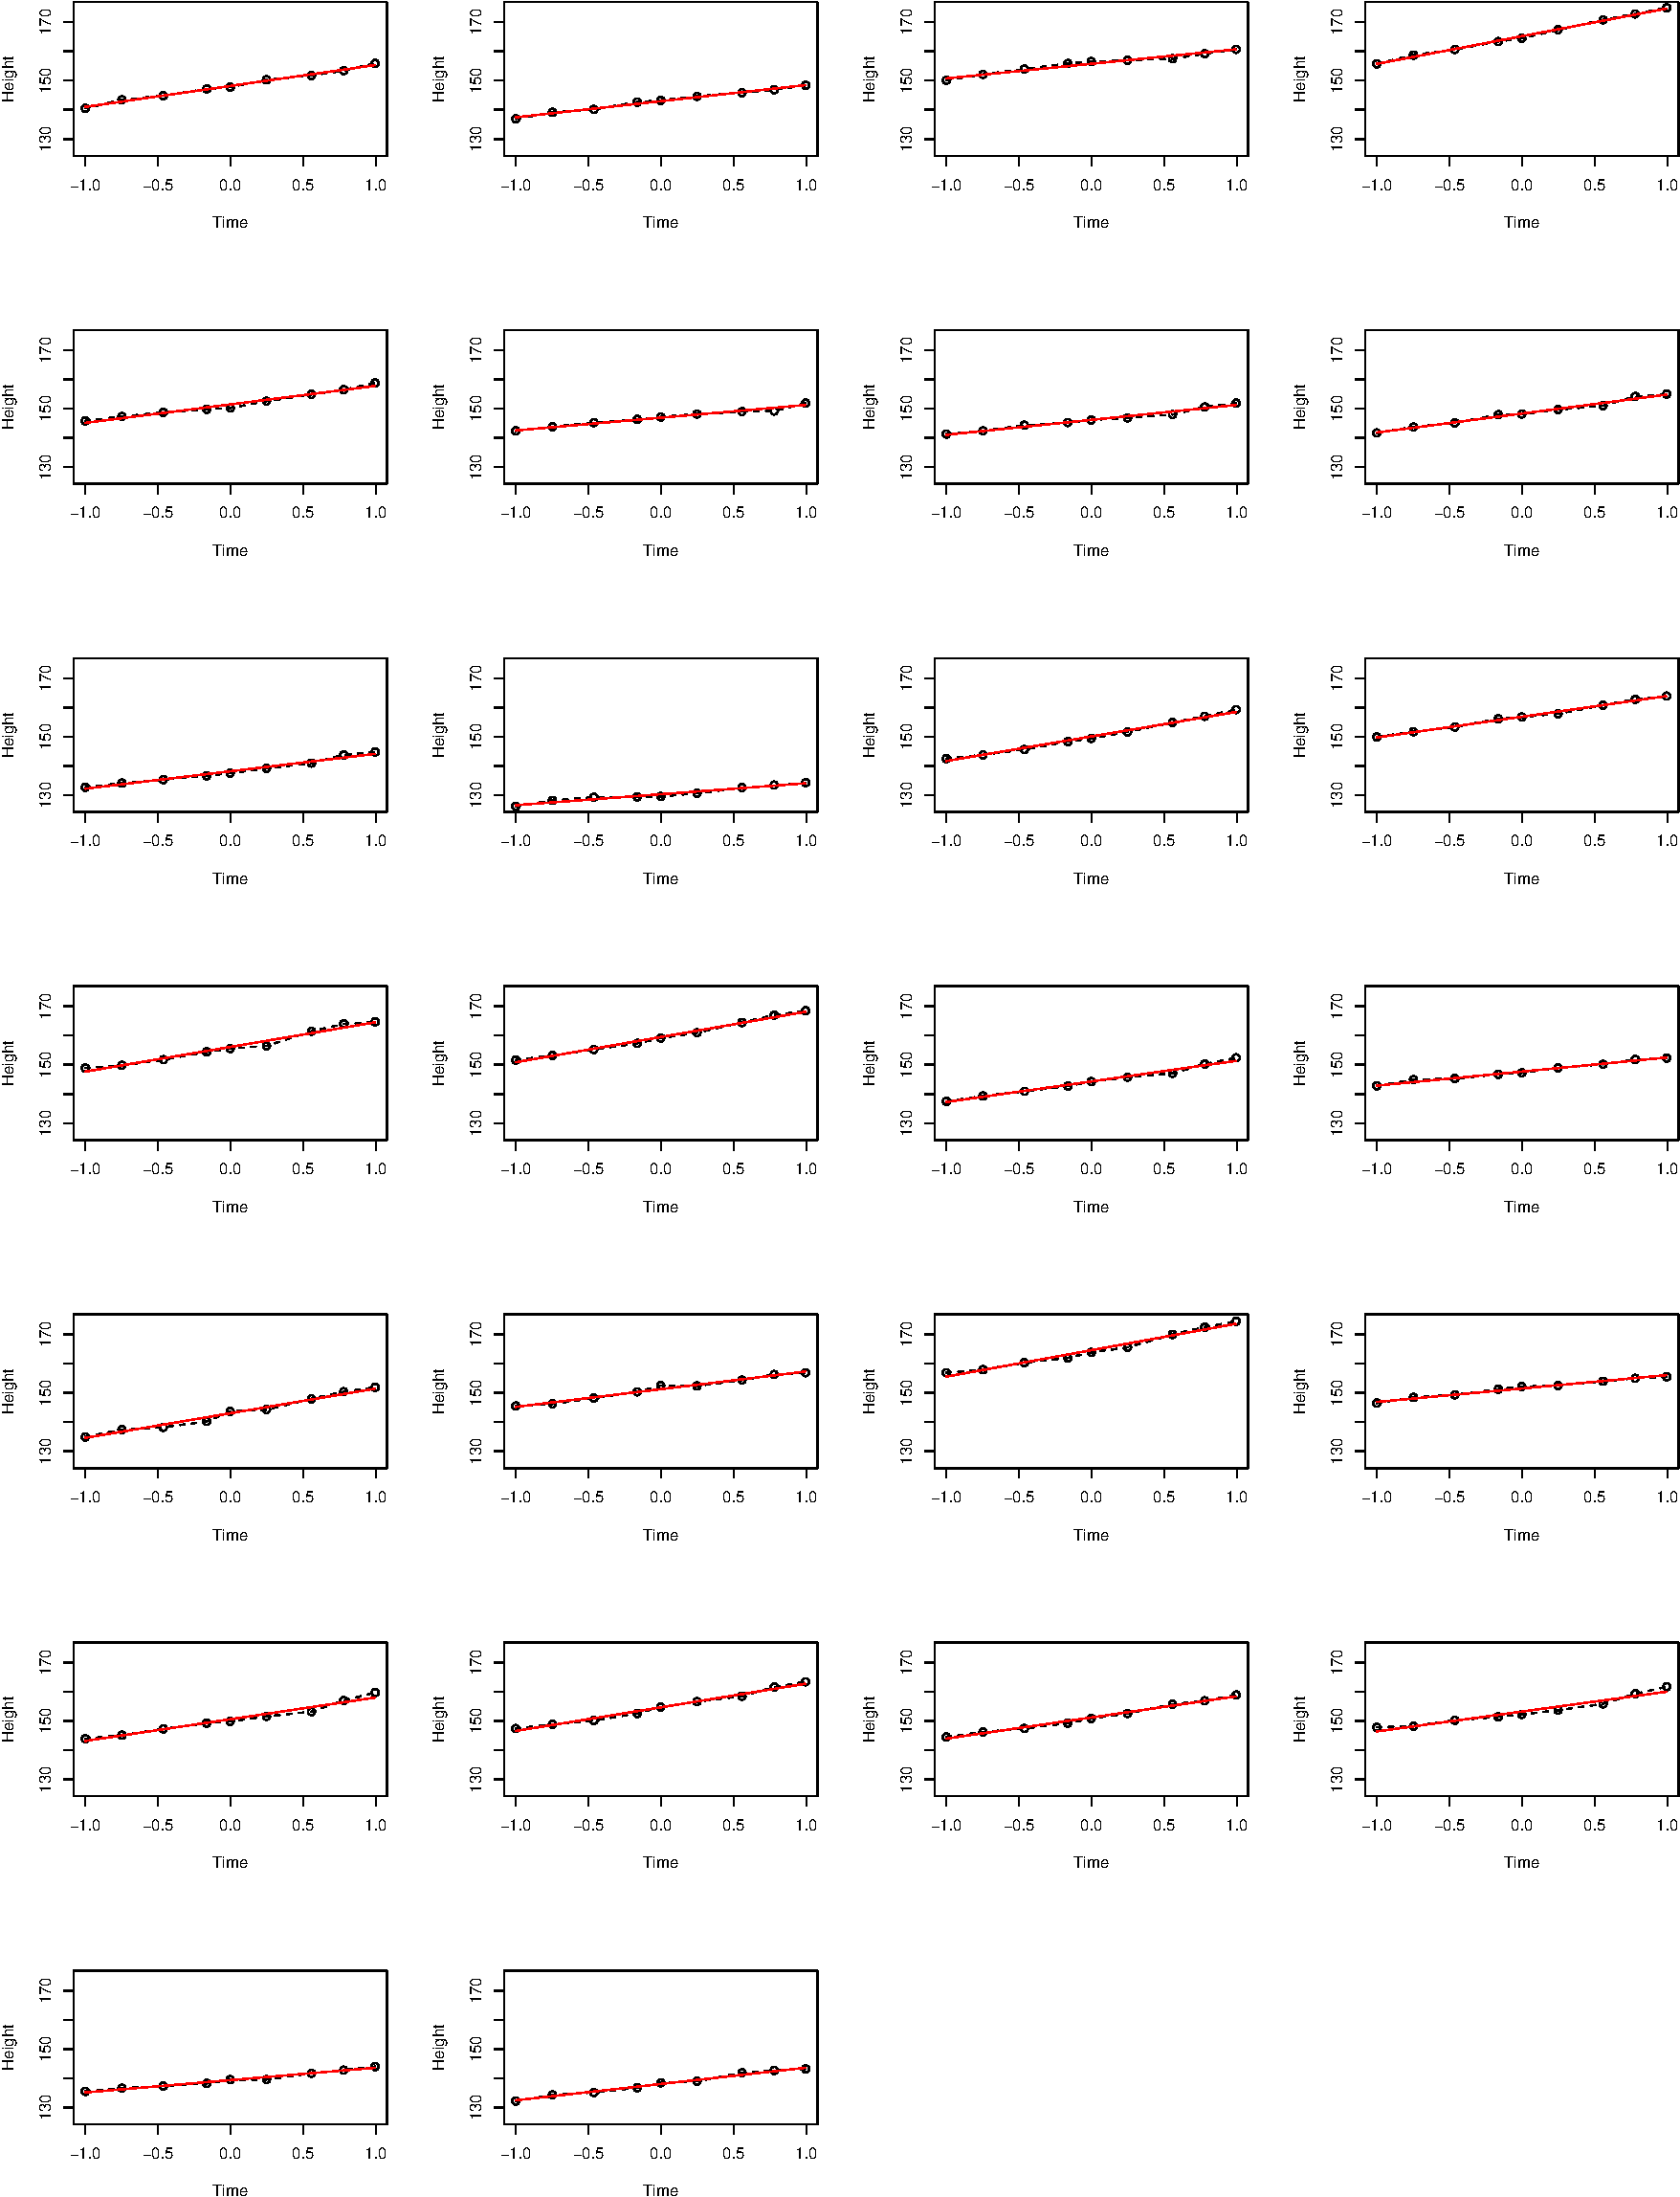
\includegraphics[width=1\linewidth]{finalexam_files/figure-latex/ex5-final-fig-1} 

}

\caption{Observed heights in data (dots, dashed line) and the model projection (red line).}\label{fig:ex5-final-fig}
\end{figure}

\end{document}
